% Dokumentenkopf ---------------------------------------------------------------
%   Diese Vorlage basiert auf "scrreprt" aus dem koma-script.
% ------------------------------------------------------------------------------
\documentclass[
    12pt,					% Schriftgröße
    DIV10,
    ngerman,				% f\"ur Umlaute, Silbentrennung etc.
    a4paper,				% Papierformat
%    numbers = noenddot	% Kein Punkt nach der letzten Ziffer in der Nummerierung
%
%    oneside,				% einseitiges Dokument
    twoside,				% zweiseitiges Dokument
    openright,
    titlepage,				% es wird eine Titelseite verwendet
    parskip=half,			% Abstand zwischen Abs\"atzen (halbe Zeile)
    headings=normal,		% Gr\"o\ss e der \"uberschriften verkleinern
    %listof=totoc,			% Verzeichnisse im Inhaltsverzeichnis auff\"uhren
    %bibliography=totoc,	% Literaturverzeichnis im Inhaltsverzeichnis auff\"uhren
    %index=totoc,			% Index im Inhaltsverzeichnis auff\"uhren
    %captions=tableheading,	% Beschriftung von Tabellen oberhalb ausgeben
    %listof=flat,
    final					% Status des Dokuments (final/draft)
]{scrreprt}					% 

% Meta-Informationen -----------------------------------------------------------
%   Informationen \"uber das Dokument, wie z.B. Titel, Autor, Matrikelnr. etc
%   werden in der Datei Meta.tex definiert und k\"onnen danach global
%   verwendet werden.
% ------------------------------------------------------------------------------
% Meta-Informationen -----------------------------------------------------------
%   Definition von globalen Parametern, die im gesamten Dokument verwendet
%   werden k�nnen (z.B auf dem Deckblatt etc.).
%
%   ACHTUNG: Wenn die Texte Umlaute oder ein Esszet enthalten, muss der folgende
%            Befehl bereits an dieser Stelle aktiviert werden:
%            \usepackage[latin1]{inputenc}
% ------------------------------------------------------------------------------
\newcommand{\titel}{Titel der Masterarbeit}
\newcommand{\untertitel}{und hier kommt der Untertitel}
\newcommand{\art}{Masterarbeit}
\newcommand{\fachgebiet}{Software-Engineering}
\newcommand{\autor}{Hans Meier}
\newcommand{\studienbereich}{Software-Engineering}
\newcommand{\matrikelnr}{12 34 56}
\newcommand{\erstgutachter}{Prof. Dr. Werner Berentzen}
\newcommand{\zweitgutachter}{Dipl.-Inf. Lukas Podolski}
\newcommand{\jahr}{2009}
\newcommand{\ort}{Berlin}
\newcommand{\logo}{LogoOhmHochschule.jpg}


% ben\"otigte Packages -----------------------------------------------------------
%   LaTeX-Packages, die ben\"otigt werden, sind in die Datei Packages.tex
%   "ausgelagert", um diese Vorlage m\"oglichst \"ubersichtlich zu halten.
% ------------------------------------------------------------------------------
% Anpassung des Seitenlayouts --------------------------------------------------
%   siehe Seitenstil.tex
% ------------------------------------------------------------------------------
\usepackage[
    automark, % Kapitelangaben in Kopfzeile automatisch erstellen
    headsepline, % Trennlinie unter Kopfzeile
    ilines % Trennlinie linksb�ndig ausrichten
]{scrpage2}

% Anpassung an Landessprache ---------------------------------------------------
\usepackage[ngerman]{babel}

% Umlaute ----------------------------------------------------------------------
%   Umlaute/Sonderzeichen wie ���� direkt im Quelltext verwenden (CodePage).
%   Erlaubt automatische Trennung von Worten mit Umlauten.
% ------------------------------------------------------------------------------
\usepackage[latin1]{inputenc}
\usepackage[T1]{fontenc}
\usepackage{textcomp} % Euro-Zeichen etc.

% Schrift ----------------------------------------------------------------------
\usepackage{lmodern} % bessere Fonts
\usepackage{relsize} % Schriftgr��e relativ festlegen

% Grafiken ---------------------------------------------------------------------
% Einbinden von JPG-Grafiken erm�glichen
\usepackage[dvips,final]{graphicx}
% hier liegen die Bilder des Dokuments
\graphicspath{{Bilder/}}

% Befehle aus AMSTeX f�r mathematische Symbole z.B. \boldsymbol \mathbb --------
\usepackage{amsmath,amsfonts}

% f�r Index-Ausgabe mit \printindex --------------------------------------------
\usepackage{makeidx}

% Einfache Definition der Zeilenabst�nde und Seitenr�nder etc. -----------------
\usepackage{setspace}
\usepackage{geometry}

% Symbolverzeichnis ------------------------------------------------------------
%   Symbolverzeichnisse bequem erstellen. Beruht auf MakeIndex:
%     makeindex.exe %Name%.nlo -s nomencl.ist -o %Name%.nls
%   erzeugt dann das Verzeichnis. Dieser Befehl kann z.B. im TeXnicCenter
%   als Postprozessor eingetragen werden, damit er nicht st�ndig manuell
%   ausgef�hrt werden muss.
%   Die Definitionen sind ausgegliedert in die Datei "Glossar.tex".
% ------------------------------------------------------------------------------
\usepackage[intoc]{nomencl}
\let\abbrev\nomenclature
\renewcommand{\nomname}{Abk�rzungsverzeichnis}
\setlength{\nomlabelwidth}{.25\hsize}
\renewcommand{\nomlabel}[1]{#1 \dotfill}
\setlength{\nomitemsep}{-\parsep}

% zum Umflie�en von Bildern ----------------------------------------------------
\usepackage{floatflt}


% zum Einbinden von Programmcode -----------------------------------------------
\usepackage{listings}
\usepackage{xcolor} 
\definecolor{hellgelb}{rgb}{1,1,0.9}
\definecolor{colKeys}{rgb}{0,0,1}
\definecolor{colIdentifier}{rgb}{0,0,0}
\definecolor{colComments}{rgb}{1,0,0}
\definecolor{colString}{rgb}{0,0.5,0}
\lstset{
    float=hbp,
    basicstyle=\ttfamily\color{black}\small\smaller,
    identifierstyle=\color{colIdentifier},
    keywordstyle=\color{colKeys},
    stringstyle=\color{colString},
    commentstyle=\color{colComments},
    columns=flexible,
    tabsize=2,
    frame=single,
    extendedchars=true,
    showspaces=false,
    showstringspaces=false,
    numbers=left,
    numberstyle=\tiny,
    breaklines=true,
    backgroundcolor=\color{hellgelb},
    breakautoindent=true
}

% URL verlinken, lange URLs umbrechen etc. -------------------------------------
\usepackage{url}

% wichtig f�r korrekte Zitierweise ---------------------------------------------
\usepackage[square]{natbib}

% PDF-Optionen -----------------------------------------------------------------
\usepackage[
    bookmarks,
    bookmarksopen=true,
    colorlinks=true,
% diese Farbdefinitionen zeichnen Links im PDF farblich aus
    linkcolor=red, % einfache interne Verkn�pfungen
    anchorcolor=black,% Ankertext
    citecolor=blue, % Verweise auf Literaturverzeichniseintr�ge im Text
    filecolor=magenta, % Verkn�pfungen, die lokale Dateien �ffnen
    menucolor=red, % Acrobat-Men�punkte
    urlcolor=cyan, 
% diese Farbdefinitionen sollten f�r den Druck verwendet werden (alles schwarz)
    %linkcolor=black, % einfache interne Verkn�pfungen
    %anchorcolor=black, % Ankertext
    %citecolor=black, % Verweise auf Literaturverzeichniseintr�ge im Text
    %filecolor=black, % Verkn�pfungen, die lokale Dateien �ffnen
    %menucolor=black, % Acrobat-Men�punkte
    %urlcolor=black, 
    backref,
    plainpages=false, % zur korrekten Erstellung der Bookmarks
    pdfpagelabels, % zur korrekten Erstellung der Bookmarks
    hypertexnames=false, % zur korrekten Erstellung der Bookmarks
    linktocpage % Seitenzahlen anstatt Text im Inhaltsverzeichnis verlinken
]{hyperref}
% Befehle, die Umlaute ausgeben, f�hren zu Fehlern, wenn sie hyperref als Optionen �bergeben werden
\hypersetup{
    pdftitle={\titel \untertitel},
    pdfauthor={\autor},
    pdfcreator={\autor},
    pdfsubject={\titel \untertitel},
    pdfkeywords={\titel \untertitel},
}

% fortlaufendes Durchnummerieren der Fu�noten ----------------------------------
\usepackage{chngcntr}

% f�r lange Tabellen -----------------------------------------------------------
\usepackage{longtable}
\usepackage{array}
\usepackage{ragged2e}
\usepackage{lscape}

% Spaltendefinition rechtsb�ndig mit definierter Breite ------------------------
\newcolumntype{w}[1]{>{\raggedleft\hspace{0pt}}p{#1}}

% Formatierung von Listen �ndern -----------------------------------------------
\usepackage{paralist}

% bei der Definition eigener Befehle ben�tigt
\usepackage{ifthen}

% definiert u.a. die Befehle \todo und \listoftodos
\usepackage{todonotes}

% sorgt daf�r, dass Leerzeichen hinter parameterlosen Makros nicht als Makroendezeichen interpretiert werden
\usepackage{xspace}


% Hyperlinks, Seitenränder etc. ---------------------------------------
%% PDF-Optionen -----------------------------------------------------------------
\usepackage{scrhack}
\usepackage[
    bookmarks=true,
    bookmarksopen=true,
    colorlinks=true,
% diese Farbdefinitionen zeichnen Links im PDF farblich aus
%    linkcolor=black, % einfache interne Verknüpfungen
%    anchorcolor=black,% Ankertext
%    citecolor=blue, % Verweise auf Literaturverzeichniseinträge im Text
%    filecolor=magenta, % Verknüpfungen, die lokale Dateien öffnen
%    menucolor=red, % Acrobat-Menüpunkte
%    urlcolor=cyan, 
% diese Farbdefinitionen sollten für den Druck verwendet werden (alles schwarz)
    linkcolor=black, % einfache interne Verknüpfungen
    anchorcolor=black, % Ankertext
    citecolor=black, % Verweise auf Literaturverzeichniseintröge im Text
    filecolor=black, % Verknüpfungen, die lokale Dateien öffnen
    menucolor=black, % Acrobat-Menüpunkte
    urlcolor=black,
% andere Def. für Hyperlinks
    pdftex,
    pdfnewwindow = true,
    pagebackref = false,
    plainpages=false, % zur korrekten Erstellung der Bookmarks
    pdfpagelabels=true, % zur korrekten Erstellung der Bookmarks
    hypertexnames=true, % zur korrekten Erstellung der Bookmarks
    breaklinks=true, % zur korrekten Erstellung der Bookmarks
    linktocpage % Seitenzahlen anstatt Text im Inhaltsverzeichnis verlinken
]{hyperref}

\usepackage[all]{hypcap}

% Befehle, die Umlaute ausgeben, führen zu Fehlern, wenn sie hyperref als Optionen übergeben werden
\hypersetup{
    pdftitle={\titel},
    pdfauthor={\autor},
    pdfproducer={\LaTeX},
    pdfcreator={\LaTeX},
    pdfsubject={\titel\ - \untertitel},
    pdfkeywords={\titel\ - \untertitel},
}

% Zeilenabstand 1,5 Zeilen -----------------------------------------------------
\onehalfspacing

% Seitenränder -----------------------------------------------------------------
\setlength{\topskip}{\ht\strutbox} % behebt Warnung von geometry
\geometry{
	paper=a4paper,
	bindingoffset=10mm,
	left=15mm,
	right=25mm,
	top=20mm,
	bottom=35mm,
	headsep=5mm,
	footskip=10mm,
}
% PDF-Optionen -----------------------------------------------------------------
\usepackage{scrhack}
\usepackage[
    bookmarks=true,
    bookmarksopen=true,
    colorlinks=true,
% diese Farbdefinitionen zeichnen Links im PDF farblich aus
    linkcolor=black, % einfache interne Verkn\"upfungen
    anchorcolor=black,% Ankertext
    citecolor=blue, % Verweise auf Literaturverzeichniseintr\"age im Text
    filecolor=magenta, % Verkn\"upfungen, die lokale Dateien \"offnen
    menucolor=red, % Acrobat-Men\"upunkte
    urlcolor=cyan, 
% diese Farbdefinitionen sollten f\"ur den Druck verwendet werden (alles schwarz)
    %linkcolor=black, % einfache interne Verkn\"upfungen
    %anchorcolor=black, % Ankertext
    %citecolor=black, % Verweise auf Literaturverzeichniseintr\"age im Text
    %filecolor=black, % Verkn\"upfungen, die lokale Dateien \"offnen
    %menucolor=black, % Acrobat-Men\"upunkte
    %urlcolor=black,
% andere Def. für Hyperlinks
    pdftex,
    pdfnewwindow = true,
    pagebackref = false,
    plainpages=false, % zur korrekten Erstellung der Bookmarks
    pdfpagelabels=true, % zur korrekten Erstellung der Bookmarks
    hypertexnames=true, % zur korrekten Erstellung der Bookmarks
    breaklinks=true, % zur korrekten Erstellung der Bookmarks
    linktocpage % Seitenzahlen anstatt Text im Inhaltsverzeichnis verlinken
]{hyperref}

\usepackage[all]{hypcap}

% Befehle, die Umlaute ausgeben, f\"uhren zu Fehlern, wenn sie hyperref als Optionen \"ubergeben werden
\hypersetup{
    pdftitle={\titel},
    pdfauthor={\autor},
    pdfproducer={\LaTeX},
    pdfcreator={\LaTeX},
    pdfsubject={\titel\ - \untertitel},
    pdfkeywords={\titel\ - \untertitel},
}

% Zeilenabstand 1,5 Zeilen -----------------------------------------------------
\onehalfspacing

% Seitenränder -----------------------------------------------------------------
\setlength{\topskip}{\ht\strutbox} % behebt Warnung von geometry
\geometry{
	paper=a4paper,
	bindingoffset=0mm,
	left=25mm,
	right=25mm,
	top=20mm,
	bottom=35mm,
	headsep=5mm,
	footskip=10mm,
}

% Kopf- und Fu\ss zeilen, etc. ---------------------------------------
% Zeilenabstand 1,5 Zeilen -----------------------------------------------------
\onehalfspacing

% Seitenr�nder -----------------------------------------------------------------
\setlength{\topskip}{\ht\strutbox} % behebt Warnung von geometry
\geometry{paper=a4paper,left=35mm,right=35mm,top=30mm}

% Kopf- und Fu�zeilen ----------------------------------------------------------
\pagestyle{scrheadings}
% Kopf- und Fu�zeile auch auf Kapitelanfangsseiten
\renewcommand*{\chapterpagestyle}{scrheadings} 
% Schriftform der Kopfzeile
\renewcommand{\headfont}{\normalfont}

% Kopfzeile
\ihead{\large{\textsc{\titel}}\\ \small{\untertitel} \\[2ex] \textit{\headmark}}
\chead{}
\ohead{\includegraphics[scale=0.15]{\logo}}
\setlength{\headheight}{21mm} % H�he der Kopfzeile
% Kopfzeile �ber den Text hinaus verbreitern
\setheadwidth[0pt]{textwithmarginpar} 
\setheadsepline[text]{0.4pt} % Trennlinie unter Kopfzeile

% Fu�zeile
\ifoot{\copyright\ \autor}
\cfoot{}
\ofoot{\pagemark}

% sonstige typographische Einstellungen ----------------------------------------

% erzeugt ein wenig mehr Platz hinter einem Punkt
\frenchspacing 

% Schusterjungen und Hurenkinder vermeiden
\clubpenalty = 10000
\widowpenalty = 10000 
\displaywidowpenalty = 10000

% Quellcode-Ausgabe formatieren
\lstset{numbers=left, numberstyle=\tiny, numbersep=5pt, breaklines=true}
\lstset{emph={square}, emphstyle=\color{red}, emph={[2]root,base}, emphstyle={[2]\color{blue}}}

% Fu�noten fortlaufend durchnummerieren
\counterwithout{footnote}{chapter}


% eigene Definitionen f\"ur Silbentrennung
% Trennvorschl�ge im Text werden mit \" angegeben
% untrennbare W�rter und Ausnahmen von der normalen Trennung k�nnen in dieser
% Datei mittels \hyphenation definiert werden


% eigene LaTeX-Befehle
% Eigene Befehle und typographische Auszeichnungen für diese
%\addtocontents{toc}{\protect\newpage} %Seitenumbruch in Inhaltsverzeichnis erzwingen

% einfaches Wechseln der Schrift, z.B.: \changefont{cmss}{sbc}{n}
%\newcommand{\changefont}[3]{\fontfamily{#1} \fontseries{#2} \fontshape{#3} \selectfont}

% Abkürzungen mit korrektem Leerraum 
\newcommand{\sa}{\mbox{s.\,a.\ }}
\newcommand{\ua}{\mbox{u.\,a.\ }}
\newcommand{\zB}{\mbox{z.\,B.\ }}
\newcommand{\dahe}{\mbox{d.\,h.\ }}
\newcommand{\Vgl}{Vgl.\ }
\newcommand{\vgl}{vgl.\ }
\newcommand{\bzw}{bzw.\ }
\newcommand{\uvm}{uvm.\ }
\newcommand{\evtl}{evtl.\ }

\newcommand{\abbildung}[1]{Abbildung~\ref{fig:#1}}

\newcommand{\bs}{$\backslash$}
%\newcommand{\bs}[1]{\boldsymbol{#1}}

% erzeugt ein Listenelement mit fetter Überschrift 
\newcommand{\itemd}[2]{\item{\textbf{#1}}\\{#2}}

% einige Befehle zum Zitieren --------------------------------------------------
\newcommand{\Zitat}[2][\empty]{\ifthenelse{\equal{#1}{\empty}}{\citep{#2}}{\citep[#1]{#2}}}

% zum Ausgeben von Autoren
\newcommand{\AutorName}[1]{\textsc{#1}}
\newcommand{\Autor}[1]{\AutorName{\citeauthor{#1}}}

% verschiedene Befehle um Wörter semantisch auszuzeichnen ----------------------
\newcommand{\NeuerBegriff}[1]{\textbf{#1}}
\newcommand{\Fachbegriff}[1]{\textit{#1}}

\newcommand{\Eingabe}[1]{\texttt{#1}}
%\newcommand{\Code}[1]{\texttt{#1}}
\newcommand{\Datei}[1]{\texttt{#1}}

\newcommand{\Datentyp}[1]{\textsf{#1}}
\newcommand{\XMLElement}[1]{\textsf{#1}}
\newcommand{\Webservice}[1]{\textsf{#1}}

% verschiedene Befehle um Wörter semantisch auszuzeichnen ----------------------
\newcommand{\Index}[1]{#1\index{#1}}

%\newcommand{\Quelle}{\footnotesize Quelle: }
\newcommand{\Quelle}[1]{\footnotesize{}Quelle: #1}
% im Index erscheinen alle gepunkteten Linien direkt \"ubereinander
\renewcommand{\dotfill}{\leaders\hbox to2mm{\hss.\hss}\hskip 2mm plus1fill}
%\renewcommand{\dotfill}{\leaders\hbox to 5p1{\hss.\hss}\hfill}

% alternativ on-the-fly Konvertierung beim Übersetzungsvorgang wird externer Grafikkonverter aufgerufen
%\DeclareGraphicsRule{.jpg}{.eps}{}{jpeg2ps #1}

% Das eigentliche Dokument -----------------------------------------------------
%   Der eigentliche Inhalt des Dokuments beginnt hier. Die einzelnen Seiten
%   und Kapitel werden in eigene Dateien ausgelagert und hier nur inkludiert.
% ------------------------------------------------------------------------------
\begin{document}
% auch subsubsection nummerieren
\setcounter{secnumdepth}{2}
\setcounter{tocdepth}{4}
\setcounter{lofdepth}{2}

% Deckblatt und Abstract ohne Seitenzahl
\ofoot{}

\thispagestyle{plain}
\begin{titlepage}

\begin{center}

\huge{\textbf{\titel}}\\[1.5ex]
\LARGE{\textbf{\untertitel}}\\[6ex]
\LARGE{\textbf{\art}}\\[1.5ex]
\Large{im Fachgebiet \fachgebiet}\\[18ex]


\includegraphics[scale=0.2]{LogoOhmHochschuleMitText.jpg}\\[6ex]

\normalsize
\begin{tabular}{w{5.4cm}p{6cm}}\\
vorgelegt von:  & \quad \autor\\[1.2ex]
Studienbereich: & \quad \studienbereich\\[1.2ex]
Matrikelnummer: & \quad \matrikelnr\\[1.2ex]
Erstgutachter:  & \quad \erstgutachter\\[1.2ex]
Zweitgutachter: & \quad \zweitgutachter\\[3ex]
\end{tabular}

\copyright\ \jahr\\[9ex]

\end{center}

\singlespacing
\small
\noindent Dieses Werk einschlie�lich seiner Teile ist \textbf{urheberrechtlich gesch�tzt}. Jede Verwertung au�erhalb der engen Grenzen des Urheberrechtgesetzes ist ohne Zustimmung des Autors unzul�ssig und strafbar. Das gilt insbesondere f�r Vervielf�ltigungen, �bersetzungen, Mikroverfilmungen sowie die Einspeicherung und Verarbeitung in elektronischen Systemen.

\end{titlepage}

\cleardoublepage
%\newpage \thispagestyle{empty} \quad \newpage

\ofoot{\pagemark}

% Seitennummerierung -----------------------------------------------------------
%   Vor dem Hauptteil werden die Seiten in gro\ss en r\"omischen Ziffern 
%   nummeriert.
% ------------------------------------------------------------------------------
\pagenumbering{Roman}
\clearpage\markboth{Kurzfassung / Abstract}{Kurzfassung / Abstract} % f�r korrekte �berschrift in der Kopfzeile
\subsubsection{Kurzfassung}

Die folgende Arbeit beschäftigt sich mit aktuellen Technologien in den Bereichen Web, 3D und Spieleentwicklung. Als Anwendung dieser Themenbereiche wurde ein klassisches Spiel aus den 1980er Jahren analysiert um die Umsetzbarkeit im Umfeld des Web zu prüfen.\\
Mit den Ergebnissen wurde anschließend eine Realisierung des Spiels durchgeführt.

\cleardoublepage

% Inhaltsverzeichnis ----------------------------------------------------------
\clearpage\markboth{\contentsname}{\contentsname} % f�r korrekte �berschrift in der Kopfzeile
\phantomsection
\addcontentsline{toc}{chapter}{\contentsname}
\tableofcontents % Inhaltsverzeichnis
\cleardoublepage

% Vorwort ----------------------------------------------------------------------
\clearpage\markboth{Vorwort}{Vorwort} % f�r korrekte �berschrift in der Kopfzeile
\chapter*{Vorwort}
\label{cha:Vorwort}
\addcontentsline{toc}{chapter}{\nameref{cha:Vorwort}}

Blabla \todo{Am Ende ausführen}
\cleardoublepage
%\newpage \thispagestyle{empty} \quad \newpage
% ------------------------------------------------------------------------------

% Selbständigkeitserklärung ----------------------------------------------------
\addchap{Eidesstattliche Erkl�rung}
Ich, \autor, Matrikel-Nr.\ \matrikelnr, versichere hiermit, dass ich meine Masterarbeit mit dem Thema
\begin{quote}
\textit{\titel} \textit{\untertitel}
\end{quote}
selbst�ndig verfasst und keine anderen als die angegebenen Quellen und Hilfsmittel benutzt habe, wobei ich alle w�rtlichen und sinngem��en Zitate als solche gekennzeichnet habe. Die Arbeit wurde bisher keiner anderen Pr�fungsbeh�rde vorgelegt und auch nicht ver�ffentlicht.

Mir ist bekannt, dass ich meine Masterarbeit zusammen mit dieser Erkl�rung fristgem�� nach Vergabe des Themas in dreifacher Ausfertigung und gebunden im Pr�fungsamt der Ohm-Hochschule abzugeben oder sp�testens mit dem Poststempel des Tages, an dem die Frist abl�uft, zu senden habe.\\[6ex]

\ort, den \today


\rule[-0.2cm]{5cm}{0.5pt}

\textsc{\autor} 

\cleardoublepage
% ------------------------------------------------------------------------------

% arabische Seitenzahlen im Hauptteil ------------------------------------------
\clearpage % neue Seite
\newcounter{tocPage} % neuer Seitenzähler
\setcounter{tocPage}{\value{page}} % eigener Seitenzähler erhöht
\pagenumbering{arabic}
\setlength{\parindent}{15pt}

% die Inhaltskapitel werden inkludiert -----------------------------------------
\chapter{Einleitung}
\label{cha:Einleitung}

\emph{Die Einleitung soll hier nur in ihrer Struktur erkl\"art werden, die anderen Unterteile f\"uhren an das Thema heran, erkl\"aren es und beschreiben den Aufbau der restlichen Arbeit}

\section{Hinführung}
\label{sec:hinfuhrung}\index{Hinführung}

\emph{Die Hinf\"uhrung soll den Leser an das Thema 3D-Technologien, Web-Entwicklung und Spieleklassiker, wie Archon heranführen. Hier sind Quellen und Recherchen zu ein paar Zahlen, wie Remakes, Umsätze zu Uralt-Spielen aktuell und Beliebtheit/Zahlen zum Webbrowser als Spieleplattform angebracht, um Wichtigkeit der Plattform und Technologien, aber auch Relevanz für Spieleklassiker zu zeigen.}

\section{Aktueller Forschungsstand}
\label{sec:aktueller_forschungsstand}\index{Forschungsstand}

\emph{Hier sollen dann Extrema zum einen in Richtung 3D-Entwicklung, in Richtung Web-Entwicklung und aber auch bei der Spiele-Entwicklung kurz herausgearbeitet werden, um dem Leser einen kurzen Einblick in aktuelle M\"oglichkeiten zu geben, und zu zeigen, dass die Arbeit "State of the Art" ist. }

\section{Motivation}
\label{sec:motivation}\index{Motivation}
\emph{ Diese Sektion soll vom vorherigen Stand der Forschung und Möglichkeiten auf Anwendbarkeit überleiten und zeigen, dass die evtl. surreal erscheinende Vermixung von Genres, Plattformen und Technologien anwendbar ist, und das sogar mit beschränktem Aufwand. }

\section{Ziele dieser Arbeit}
\label{sec:ziele_dieser_arbeit}\index{Ziele}

\emph{Hier soll bloß kurz und prägnant die Fragestellung genannt werden und eine kurze Analyse der einzelnen Worte des Titels stattfinden.}
\todo{Hier fehlt irgendwie direkt mal eine sinnvolle \"Uberleitung/Reihenfolge von Motivation zu Ziele zu zentrale Begriffe.}

\section{Zentrale Begriffe}
\label{sec:zentrale_begriffe}\index{Zentrale Begriffe}

\emph{?????}

\section{Aufbau}
\label{sec:aufbau}\index{Aufbau}

\emph{Hier wird dann auf den Aufbau des Haupt- und Schlussteils eingegangen. Also der erste Abschnitt beschäftigt sich mit Anforderungsanalyse beider Plattformen/Seiten. Der zweite Abschnitt dreht sich dann rund um Zusammenf\"uhrung der Anforderungen und Tool-Auswahl, und somit darum einen Einstiegspunkt und eine Architektur f\"ur die weitere Entwicklung festzulegen. }
% !TeX root = ../Bachelorarbeit.tex
\chapter{Hauptteil}
\label{cha:Hauptteil}

\section{Einleitung}

\section{Analyse}
\label{sec:analyse}\index{Analyse}

The goal of every video game is to present the user(s) with a situation, accept their input, interpret those signals into actions, and calculate a new situation resulting from those acts. Games are constantly looping through these stages, over and over, until some end condition occurs (such as winning, losing, or exiting to go to bed). Not surprisingly, this pattern corresponds to how a game engine is programmed. The specifics depend on the game. \cite{https://developer.mozilla.org/en-us/docs/games/anatomy}

\emph{In diesem Abschnitt soll die Vorgehensweise bei der Analyse kurz aufgezeigt werden und der Inhalt der einzelnen Teile klar gemacht werden. Also, zum einen, dass hier eben eine Anforderungsanalyse stattfindet, und zum Anderen, dass diese Analyse zweigeteilt ist.}

\subsection{Analyse des klassischen Spiels}
\label{subsec:spiel_analyse}\index{Spiel Analyse}

\emph{Hier werden alle Aspekte des klassischen Spiels herausgearbeitet, gegliedert nach Teilen: Generelle Regeln, das Board, die Figuren, Abläufe und Wirkungen, mögliche Einstellungen\\Stichwort: Komponentendiagramm!}
\\In diesem Abschnitt werden die Anforderungen und Regeln aus Archon herausgearbeitet. Die Anforderungen und Regeln werden, der Übersicht halber, in folgende Kategorien unterteilt: 
\begin{itemize}
	\item Generelle Regeln und Ziele des Spiels
	\item Das Spielbrett
	\item Das Kampfareal
	\item Die Figuren
	\item Die Zauber
\end{itemize}
Die folgenden Abschnitte enthalten eine kurze Zusammenfassung des Spiels und seinen Inhalten und Regeln anhand der obigen Aufteilung. Anschließend wird herausgearbeitet, welche Eigenschaften eine Realisierung des Spiels inne haben muss, um das Spiel ausreichend widerzuspiegeln. 
\subsubsection{Generelle Regeln und Ziele des Spiels}
Archon ist ein Spiel, dass auf einem 9 x 9 Schachbrett stattfindet. Ähnlich wie beim Schach gibt es zwei Parteien, Licht und Dunkelheit, die sich im Wettstreit gegenüberstehen.
Die Spieler ziehen dabei immer abwechselnd ihre Figuren auf dem Spielbrett, wobei kein Zug gepasst werden kann. Jeder Spieler beginnt mit 18 Figuren, die in acht verschiedene Typen gegliedert sind. Die Figuren von Licht und Dunkelheit sind vollständig unterschiedlich. Treffen zwei Figuren auf dem Spielbrett zusammen, stehen sie sich in einem Kampfareal gegenüber. Jede Figur hat dabei ihre eigenen Lebenspunkte und ihre eigene Angriffsstärke. Der Sieger dieses Kampfes bleibt auf dem Spielbrett, während der Verlierer aus dem Spiel genommen wird. Sollte der Kampf in einem Unentschieden ausgehen, werden beide Figuren aus dem Spiel genommen.
\\Das generelle Ziel des Spiels ist es alle 5 speziellen Machtfelder gleichzeitig mit eigenen Figuren zu besetzen.
Desweiteren kann das Spiel gewonnen werden, indem alle gegenerischen Figuren besiegt werden, oder die letzte Figur mit einem Gefängnis-Zauber belegt wird.
Ein Unentschieden tritt auf wenn das Spiel zu lange passiv ist, also wenn für mindestens zwölf Züge kein Kampf stattfindet und kein Zauber gewirkt wird.\\
Das Spiel kann in folgenden Modi gestartet werden: 
\begin{itemize}
	\item Spieler gegen Spieler
	\item Spieler gegen Computer
	\item Computer gegen Computer (Demo-Modus)
\end{itemize}
Wobei der erste Spieler immer die Wahl der startenden Farbe, sowie der eigenen Farbe hat.\\Weitere Einstellmöglichkeiten gibt es nicht.

\subsubsection{Das Spielbrett}
\begin{figure}[htp]
	\centering
	\captionsetup{justification=centering}
	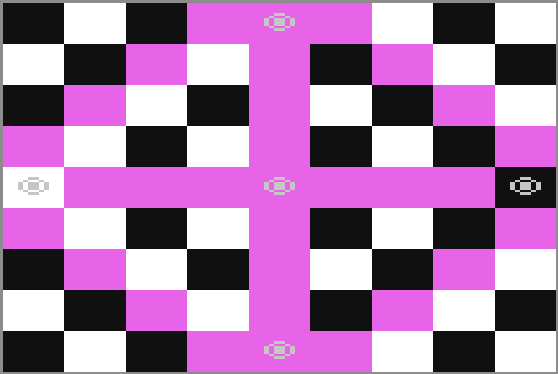
\includegraphics[width=0.50\textwidth]{ArchonStrategiieBildschirm}
	\caption[Das Spielbrett]{Das Spielbrett \footnotemark}
	\label{fig:StrategyBoard}
\end{figure}
\footnotetext{\Quelle{C64-Wiki, \url{https://www.c64-wiki.com/wiki/File:ArchonStrategiieBildschirm.gif}}}
Das Spielbrett besteht aus 9x9 Feldern von drei Typen: 
\begin{itemize}
	\item Permanent weiße Felder
	\item Permanent schwarze Felder
	\item Felder, die zwischen Schwarz, vier anderen Farben und Weiß wechseln
\end{itemize}
Alle farbwechselnden Felder ändern ihre Farbe nach dem Zug des zweiten Spielers, sodass jeder Spieler einen Zug der gleichen Farbfelder hat. Ein Farbzyklus dauert damit zwölf Züge pro Seite: Sechs von Weiß zu Schwarz und Sechs zurück.
Da sich die mittleren vier Farben je nach Ableger unterscheiden können, werden sie fortan mit Zahlen von 1 bis 6 durchnummeriert, wobei 1 Weiß darstellt und 6 Schwarz.
Wenn die Licht-Seite das Spiel beginnt, startet der Farbzyklus bei Farbe 4 und wird dunkler. Beginnt die Dunkelheit-Seite, so startet der Zyklus bei Farbe 3 und wird heller. Die Farbe der Felder gibt den darauf stehenden Figuren einen Lebenspunkte-Bonus, der größer ausfällt, je näher die Feld-Farbe an der Team-Farbe der Figur ist.
\begin{figure}[htp]
	\centering
	\captionsetup{justification=centering}
	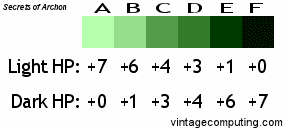
\includegraphics[width=0.40\textwidth]{archon_colorchart.png}
	\caption[Lebenspunkte-Bonus]{Lebenspunkte-Bonus anhand der Feldfarben\footnotemark}
	\label{fig:HP-Bonus}
\end{figure}
\footnote{\Quelle{vintagecomputing, \url{http://www.vintagecomputing.com/wp-content/images/archon/archon_colorchart.gif}}}
Weiterhin gibt es die fünf Machtfelder, deren Einnahme die Siegbedingung darstellt. Diese Felder haben außerdem zwei spezielle Effekte auf Figuren, die darauf stehen. Zum einen können darauf stehende Figuren -- und auch die Felder an sich, nicht Ziel eines Zaubers werden. Zum Anderen werden die Figuren nach jedem eigenen Zug um einen gewissen Betrag geheilt, sollten sie im Kampf verletzt worden sein. Diese fünf Machtfelder verteilen sich so, dass jeweils eines auf einem permanent schwarzen bzw. weißen Feld ist - dort wo der Zauberer bzw. die Zauberin ihre Ausgangsposition haben. Die anderen drei Felder sind auf farbwechselnden Feldern in der Mitte des Spielbretts verteilt.

\subsubsection{Das Kampfareal}
\begin{figure}[htp]
	\centering
	\captionsetup{justification=centering}
	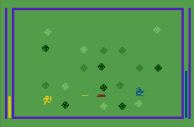
\includegraphics[width=0.40\textwidth]{archon_battlescreen_small}
	\caption[Kampfareal]{Das Kampfareal}
	\label{fig:Battlescreen}
\end{figure}
Das Kampfareal erscheint wenn zwei Figuren auf dem Spielbrett aufeinander treffen. Es stellt eine große Fläche dar, bei der von Zeit zu Zeit pflanzenähnliche Hindernisse erscheinen und wieder verschwinden. An den Seiten des Kampfareals werden die Lebenspunkte der kämpfenden Figuren in Form von Balken dargestellt.\\
Die Figuren können sich hier frei bewegen und haben, je nach Typ, unterschiedliche Eigenschaften, Attacken und Geschwindigkeiten.

\subsubsection{Die Figuren}
Das Spielbrett ist zu Spielbeginn mit 18 Spielfiguren pro Seite belegt. Es gibt 16 verschiedene Typen von Figuren, wobei die Typen von entsprechenden Figuren von Licht und Dunkelheit unterschiedlich sind. Die Beschreibung der Typen wird hier oberflächlich in Form einer Auflistung gestaltet, da die exakten Zahlenwerte der Lebenspunkte, Geschwindigkeiten und andere Eigenschaften bereits in einer anderen Zusammenfassung zu finden sind und an diesem Punkt für einen generellen Einblick in das Spiel nicht relevant sind.\footnote{Für mehr Details siehe: The secrets of Archon \url{http://www.vintagecomputing.com/index.php/archives/44}}
\begin{multicols}{2}
	Die Figuren des Lichts sind: 
	\begin{itemize}
		\item Ritter
		\item Bogenschütze
		\item Walküre
		\item Golem
		\item Einhorn
		\item Phönix
		\item Dschinn
		\item Zauberer
	\end{itemize}
\columnbreak
	Die Figuren der Dunkelheit sind:
	\begin{itemize}
		\item Goblin
		\item Mantikor
		\item Banshee
		\item Troll
		\item Basilisk
		\item Gestaltwandler
		\item Drache
		\item Zauberin
	\end{itemize}
\end{multicols}
Sich gegenüber stehende Figuren-Klassen in dieser Auflistung entsprechen sich in etwa in ihrer Stärke. Die Figuren haben dabei auch auf dem Spielbrett unterschiedliche Eigenschaften, so können Boden-Figuren, wie der Troll oder der Ritter, nicht über andere Figuren hinweg gesetzt werden und nicht diagonal bewegt werden. Je nach Typ ist die Bewegungsreichweite unterschiedlich: Drache und Dschinn können beispielsweise bis zu 4 Felder bewegt werden, während die Walküre und die Banshee nur 3 Felder bewegt werden können.\\
Außerdem kann mit Hilfe eines Zaubers einer von vier Elementaren einmal pro Seite und Spiel beschworen werden. Sollte ein Elementar beschworen werden wird er aus der Liste der möglichen Elementare entfernt, sodass niemals in einem Spiel zwei gleiche Elementare beschworen werden können. Die vier Elementare sind nach den vier Elementen Feuer, Wasser, Erde und Luft eingeteilt und besitzen, ähnlich zu normalen Figuren, unterschiedliche Sprites\footnote{Sprite - graphisches Objekt, dass vor dem Hintergrund dargestellt wird, oft auch als Shape bezeichnet} und Werte. Welcher Elementar beschworen wird ist zufällig. Weiterhin bekommen Elementare keinen Lebenspunkte-Bonus von Feldfarben, sie haben also immer die gleichen Lebenspunkte.

\subsubsection{Die Zauber}
Der Zauberer und die Zauberin können, jeweils, einmal pro Spiel die folgenden sieben Zauber wirken:
\begin{itemize}
	\itemd{Teleportieren}
	Teleportiert eine eigene Figur auf ein Feld der eigenen Wahl. Sollte das Feld belegt sein, startet direkt ein Kampf.
	\itemd{Heilen}
	Heilt eine eigene, verwundete Figur vollständig.
	\itemd{Wiederbeleben}
	Belebt eine eigene, tote Figur wieder. Die Figur muss auf eines der umliegenden Felder des Zauberers \bzw der Zauberin platziert werden, egal wo sich die Figur befindet.
	\itemd{Tauschen}
	Tauscht die Position zweier Figuren -- unabhängig ihrer Farbe.
	\itemd{Zeitumkehr}
	Dreht den Farbzyklus um. Sollten die Felder jedoch Schwarz \bzw Weiß sein wenn der Zauber gewirkt wird, ändern sie ihre Farbe zur jeweils gegenteiligen Farbe beim nächsten Farbwechsel.
	\itemd{Bewegungsunfähigkeit}
	Eine Einheit wird unfähig gemacht Bewegungen auszuführen und Zauber zu wirken. Die Einheit bleibt bewegungsunfähig bis die Farb-Felder die eigene Team-Farbe erreicht haben. Die Einheit kann sich aber weiterhin normal im Kampfareal bewegen und angreifen.
	\itemd{Elementar beschwören}
	Beschwört einen Elementar auf ein auf ein besetztes Feld, sodass direkt ein Kampf stattfindet.
\end{itemize}
Das wirken eines Zaubers ist nicht auf Machtfelder möglich. Außerdem schwächt das Wirken jedes Zaubers den Lebenspunkte-Bonus auf dem Heimat-Feld des Zauberers bzw. der Zauberin um einen Punkt, sodass nach dem Wirken aller Zauber in einem Spiel der Bonus auf null Punkte geht.

\subsubsection{Zusammenfassung für die Realisierung}
\todo{Review fällig}
Alle vorher genannten Aspekte des Spiels bilden den Kern, der das Spiel ausmacht: Ein Strategiespiel auf einem 9x9 Schachbrett mit Action-Elementen in einem Kampfareal und gut gewichteten Spielfiguren.\\
Um nun also eine ausreichende Schnittmenge mit dem Original zu haben und die neue Realisierung als "Ableger von Archon" bezeichnen zu können, sollten alle Aspekte unter "generelle Regeln und Ziele des Spiels" auf jeden Fall implementiert werden. Eine Ausnahme bildet hier die Auswahl der Spielmodi: Das Spiel an sich bietet zwar drei Modi an, jedoch ist es für eine erste Realisierung nur wichtig einen der Modi zu implementieren.\\
Das Spielbrett muss in seiner kompletten Funktionalität implementiert werden, da ganze Mechaniken sonst wegfallen und andere Mechaniken nutzlos machen. So zum Beispiel der Lebenspunkte-Bonus durch den Farbwechsel, oder die Machtfelder als Einnahmepunkte mit speziellen Funktionen.\\
Das Kampfareal kann in einer ersten Version einfach implementiert sein. Wichtig ist hier nur das Vorhandensein an sich, sowie eine entsprechende Gewichtung der einzelnen Figuren nach ihrer Kampfkraft im Original.\\
Bei den Figuren sollten zumindest einige Typen implementiert sein. Es müssen nicht alle Figuren originalgetreu nachgebildet werden, sondern es sollte eine gewichtete Auswahl von Figuren geben, sodass ein Spiel zustandekommen kann. Das Aussehen kann dabei nach belieben angepasst werden um so der Realisierung einen eigenen Charme zu geben. Wichtig ist hier, wieder einmal, nur die richtige Gewichtung von Kräften.
Die Zauber machen beim Original einen großen Teil der strategischen Mechanik aus, sodass sie vollständig zu implementieren sind. Die Zauber an kritischen Zeitpunkten im Spiel zu wirken macht Archon und jede einzelne Partie besonders. Der Stil der Zauber ist auch hier nicht wichtig, sondern ausschließlich ihre Funktion.
\subsection{Anforderungsanalyse an neue Realisierung}
\label{subsec:neueReal_analyse}\index{Analyse neue Realisierung}
\emph{Hier wird analysiert, welche Aspekte das Spiel von der Seite der technologisch gestellten Anforderungen erfüllen muss. Also: Es muss eine 3D- Engine geben, die irgendwie im Browser renderbar ist.\\ Es muss möglich sein, alle Spiel-Mechaniken mittels Server-Client-Kommunikation umzusetzen, etc.\\Stichwort: Komponentendiagramm!}\\
Der Titel, sowie die Einleitung haben schon erläutert, dass bei dieser Realisierung zwei essentielle Technologien zum Einsatz kommen sollen: \todo{Hier ist noch Arbeit nötig!}
\begin{enumerate}
	\item 3D-Technologien
	\item Web-Technologien
\end{enumerate}
Dieser Abschnitt soll nun darstellen welche Aspekte der einzelnen Spiel-Funktionalitäten durch welche Technologie umgesetzt werden kann, oder ob es \evtl Hürden auf technologischer Ebene gibt, die durch Kompromisse in der Spiel-Mechanik gelöst werden müssen.\\
\subsubsection{Web-Technologien}
Da das Spiel mittels Web-Technologien realisiert werden soll, muss jegliche Kommunikation, unabhängig vom umgesetzten Modus, mittels Server-Client-Mechanismen gelöst werden können. Die größten Anforderungen an Kommunikation stellt dabei der Action-Aspekt im Kampfareal dar. Hier wird Echtzeit-Kommunikation auf einem ziemlich hohen Niveau benötigt um möglichst kleine Latenzen zwischen Updates zu vermeiden und so das Spiel überhaupt spielbar zu machen. Als Lösung für dieses Problem bietet sich der Websocket-Standard an, der von vielen Browsern unterstützt wird. Dieser Standard ermöglicht bidirektionale, asynchrone Kommunikation, ohne dass erneute TCP-Verbindungen aufgebaut werden müssen und damit kein großer Overhead\footnote{Overhead -- In der IT-Umgebung gängiger Begriff für Meta-Daten oder Programmcode der zusätzlich zur eigentlich Funktion ausgeführt, oder versendet werden muss} entsteht. Der Client muss sich dazu einmalig mit einem Websocket unterstützenden Server verbinden. Über Websockets versendete Nachrichten können auch mit Objekten als Daten gefüllt werden, welche dann meist im JSON\footnote{JSON -- JavaScript Object Notation}-Format übertragen werden. Durch die weite Verbreitung des JSON-Formats ist die weitere Verarbeitung der Objekte stark vereinfacht und standardisiert.\\
Da Websockets, inklusive möglicher Frameworks\footnote{Framework -- softwaretechnischer Rahmen, der Funktionen und Programmstukturen bereitstellt}, in JavaScript implementiert werden ist das Dreieck der Webentwicklung die Wahl für Stil, Inhalt und Dynamisierung des Spiels.\todo{Das gefällt mir noch gar nicht.}\\
Alle anderen Aspekte des Spiels sind sehr gut vereinbar mit einem webbasierten Server-Client-Modell:
Daten können vom Server vorgehalten und, falls nötig auch gespeichert werden. Dadurch wird keine Peer-to-Peer-Kommunikation\footnote{Peer-to-Peer -- Kommunikation zwischen gleichen End-Teilnehmern ohne einen Server als Medium} nötig und alle Synchronisation von Daten geschieht über den Webserver. Die gemeinsame Datenhaltung in einer Komponente hat weiterhin den Vorteil, dass viele Überprüfungen auf Konsistenz der Daten und Regeln des Spiels ebenfalls nur an einer einzigen Stelle implementiert werden müssen.
Die weitere Dynamisierung, also auch die Reaktion auf Eingaben eines Nutzers kann durch JavaScript ausgeführt werden. Das erlaubt jede Kommunikation -- Server-Client und Spieler-Client über eine Schnittstelle abzufertigen.
Auf dem Client können Inhalte durch HTML\footnote{HTML -- Hypertext Markup Language ist eine Sprache um Dokumente im Webbrowser in ihrem Inhalt zu strukturieren }-Elemente repräsentiert und der Stil mittels CSS\footnote{CSS -- Cascading Style Sheets bilden die Regeln zum Aussehen von Webdokumenten}-Regeln angepasst werden.\\
Da aber auch 3D-Technologien in diese Realisierung einfließen sollen, bedarf es mehr als nur HTML und CSS zur Darstellung der Spielinhalte. Allein mit diesen Mitteln ist es sehr schwierig bis unmöglich teils komplexe Spielinhalte darzustellen.
\subsubsection{3D-Technologien}
Die Darstellung der Spielinhalte soll mittels 3D-Technologien stattfinden. Die Lösung für dieses Problem bieten "Canvas" und WebGL. Das HTML-Element "Canvas" ermöglicht es Inhalte im Webbrowser sehr frei zu gestalten. Das HTML-Element bietet dabei nur eine Leinwand (engl. Canvas) und die Inhalte müssen mittels JavaScript programmiert werden. Gepaart mit dem WebGL-Standard ergibt sich die Möglichkeit vielfältige, aufwändige 3D-Darstellungen im Webbrowser zu synthetisieren. Denn:  Der WebGl-Standard erlaubt es ohne Erweiterungen hardwarebeschleunigte\footnote{Hardwarebeschleunigt -- Rechenintensive Aufgaben werden vom Hauptprozessor eines Computers an dafür dedizierte Hardware delegiert, heute vermehrt Grafikkarten und grafikintensive Aufgaben} 3D-Grafiken im Browser darzustellen. WebGL-Elemente können dabei beliebig mit herkömmlichen Webseiten-Elementen, also HTML und CSS, kombiniert werden.\\

Das "Canvas"-Element bildet also die Grundlage für eine mittels WebGL programmierte Szenerie des Spiels Archon, die mit Daten aus der Echtzeitkommunikation über den WebSocket-Standard gespeist wird. Da es oberflächlich betrachtet keinerlei Showstopper, oder Einschränkungen für eine Realisierung von Archon mittels der oben genannten Technologien gibt folgt nun die Implementierung.
\section{Implementierung}
\label{sec:Umsetzung}\index{Implementierung}

\emph{Hier soll dann aufgezeigt werden, welche Anforderungen vom Spiel durch welche Technologie umgesetzt werden und nötige Bedingungen/grundsätzliche Ausschlüsse aufgezeigt werden.\\Hier, oder im nächsten Abschnitt muss klar gestellt werden, dass ein KI-Modus nicht implementiert wird!}\\
Die Implementierung von Archon wird im Folgenden gezeigt. Dabei wird zunächst betrachtet, welche Frameworks, Software-Bibliotheken, Werkzeuge und Hilfsmittel benutzt werden und welche Vereinfachungen bezüglich des Spiels getroffen werden. Anschließend wird aus den Anforderungen von Technologien und Spiel eine Grobarchitektur erstellt, die mit jedem Entwicklungsschritt verfeinert und \ggf angepasst wird.

\subsection{benötigte Technologien und Frameworks}
\label{subsec:Technologien}\index{Technologien}

\emph{Hier wird dann von den benötigten Technologien die Festlegung auf eine bestimmte Implementierung getroffen, also Frameworks, Programmiersprachen, Toolsets etc. festgelegt.}\\
Durch die bisherigen Ausarbeitungen steht fest, dass HTML, CSS und JavaScript zur Pflicht für die Implementierung des Clients werden um alle technologischen Anforderungen einhalten zu können.\\
Desweiteren gibt es aber noch Bibliotheken, die die Entwicklung des Clients beschleunigen und vereinfachen, sowie den Umgang mit Websockets und WebGL erleichtern. Außerdem muss noch die Festlegung auf einen Webserver stattfinden, der bisher lediglich der Einschränkung bedarf, dass Websockets unterstützt werden müssen.\\
Die Liste an Webservern ist ähnlich groß, wie die von Programmiersprachen. Viele grundlegende Sprachen, wie die .NET-Umgebung, C++, php \ua unterstützen dabei über Bibliotheken, oder Module auch den Websocket-Standard. Um die Entwicklung möglichst aufwandsarm zu gestalten und schnelle Fortschritte zu ermöglichen wurde sich in diesem Fall auf die node.js-Umgebung festgelegt, da hier der Server mittels JavaScript programmiert wird, was das zusätzliche Erlernen einer weiteren Programmiersprache und damit verbundene Kontext-Wechsel und Einarbeitungen in Eigenheiten, Bibliotheken und Programmiertechniken erspart.\\
Um die Entwicklung weiterhin zu beschleunigen wurde das Framework "Express" verwendet, welches es erlaubt auf einfachstem Weg über Routing-Mechanismen Webseiten-Anfragen eines Webservers zu beantworten.\\
Als Hilfsmittel für den Websocket-Standard wurde sich für Socket.io entschieden. Socket.io ist eine Library, welche Websockets wrapped und den Umgang stark vereinfacht. Socket.io erlaubt dabei eine stark Event-basierte Kommunikation, was dem Event-Emitter-Prinzip der node.js-Umgebung stark ähnelt und einen gleich Programmierstil ermöglicht. Die Library bietet ebenfalls einen Clientseitigen Teil an, welcher sich mit entsprechenden Optionen automatisch mit der Basis-Route des Webserver verbindet.\\
Für die Darstellung, also die Implementierung des WebGL-Standard wird three.js genutzt. three.js ist eine stark ausgebaute und weit verbreitete Library für Hochleistungs-3D-Entwicklung im Webbrowser. three.js besitzt weiterhin eine umfangreiche Dokumentation und eine sehr große Auswahl an Beispiel-Applikationen, welche den Einstieg und auch den weiteren Entwicklungsprozess beschleunigen.
\todo{Hier fehlt wohl noch was}\\
Die node.js-Umgebung erlaubt es sogenannte Dev-Dependencies einzufügen, also Abhängigkeiten oder Bibliotheken, welche nur im Entwicklungsprozess benutzt werden und nicht in der Produktionsversion zu finden sind. Das folgende Kapitel befasst sich daher mit Dev-Dependencies und anderen Hilftmitteln und Vereinfachungen für die Implementierung.
\subsection{Hilfsmittel und Vereinfachungen}
\label{subsec:Hilfsmittel}\index{Hilfsmittel}

\emph{Hier würden Dinge zu lesen sein, wie die Benutzung von TypeScript, oder Browser-Beschränkungen etc, da diese nicht relevant für den eigentlichen Entwicklungsvorgang sind, aber dennoch nützlich sind und eben Vereinfachungen darstellen.}

Als größte Dev-Dependency sei an dieser Stelle TypeScript zu nennen. TypeScript ist ein sogenanntes Superset zu JavaScript: Jedes valide JavaScript-Programm ist also auch ein valides TypeScript-Programm. TypeScript wird direkt zu JavaScript mittels des Compilers tsc kompiliert. TypeScript fügt zu normalem JavaScript-Code statische Typen hinzu, sodass eine statische Analyse des Codes zur Kompilierzeit auf Fehler erfolgen kann, was die Sicherheit von Schnittstellen und Funktionsaufrufen erhöht. Zu TypeScript gehören als weitere Dev-Dependency die zugehörigen Typen-Deklarationen für bereits existierende JavaScript-Bibliotheken, sodass diese auch im TypeScript korrekt erkannt und von einer IDE\footnote{Integrated Development Environment} \bzw einem Code-Editor mit Auto-Vervollständigung genutzt werden können.

\subsection{Architektur}
\label{subsec:Architektur}\index{Architektur}
Dieser Abschnitt enthält eine klassische objektorientiere Analyse des Spiels, sowie der Anforderungen aus der technologischen Sichtweise. Aus dieser Analyse soll dann eine Software-Architektur entstehen, die alle Anforderungen vereint und einen möglichst gut wartbaren und erweiterbaren Rahmen darstellt.\\
Am Anfang einer objektorientieren Analyse steht meist ein Begriffsmodell, dass grob die Beziehungen einzelner Elemente aufzeigt, ohne sich direkt auf Code-Ebene zu bewegen. Auch diese Analyse soll dem Muster folgen. 
\begin{figure}[h]
	\centering
	\captionsetup{justification=centering}
	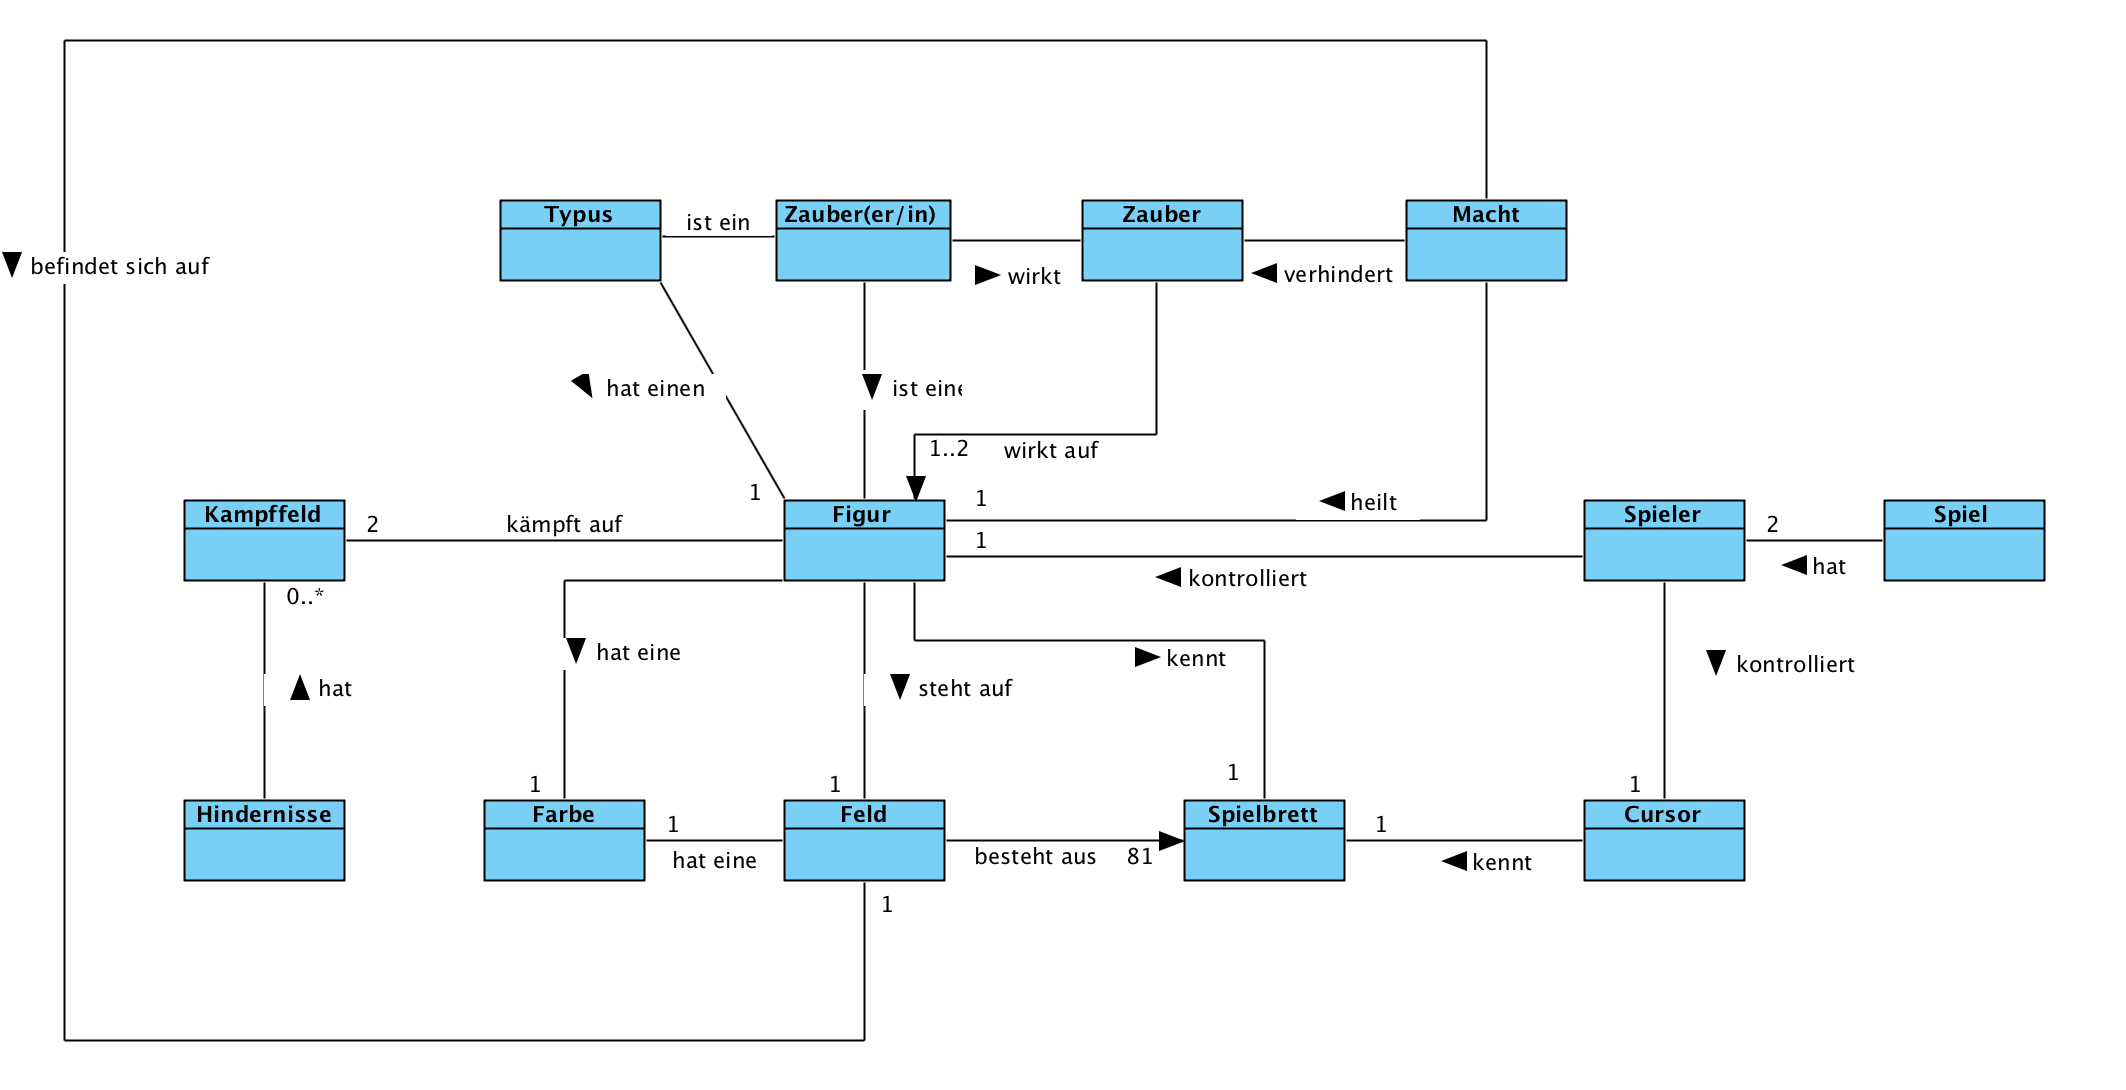
\includegraphics[width=1\textwidth]{Begriffsmodell}
	\caption[Begriffsmodell]{Begriffsmodell}
	\label{fig:Begriffsmodell}
\end{figure}
Die Abbildung \ref{fig:Begriffsmodell} stellt lediglich die im Kapitel \ref{subsec:spiel_analyse} dargestellten Inhalte grafisch dar, was aber den Entwurf und die Zusammenhänge von Klassen und Objekten im Folgenden stark erleichtert. Das Begriffsmodel ist nur für die reine Spielelogik gültig und beinhaltet noch keinerlei Ansätze für den technologischen Aspekt der Architektur! Die folgenden Abschnitte sollen daher den Entwurf der generellen Systemarchitektur näher erläutern. Dabei wird, soweit möglich, noch nicht auf externe Abhängigkeiten eingegangen und die Architektur auch möglichst frei von konkreten Festlegungen auf Technologien und Frameworks gehalten. Am Ende dieses Kapitels werden die technologischen Abhängigkeiten aufgezeigt und mit in die Architektur integriert.

\begin{figure}[htp]
	\centering
	\captionsetup{justification=centering}
	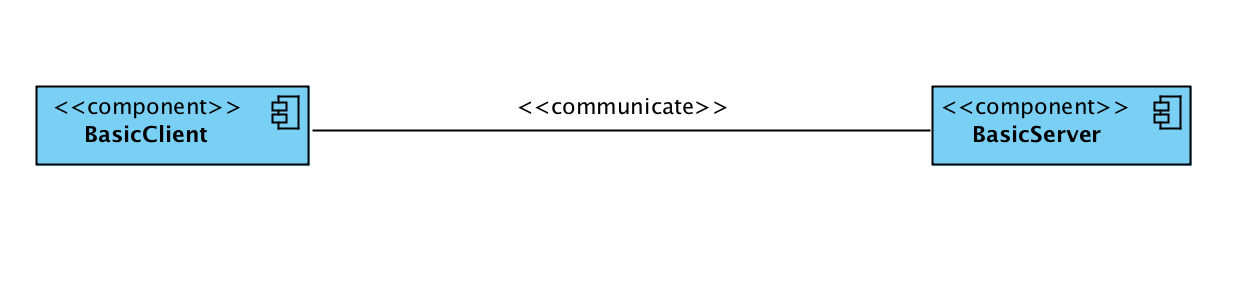
\includegraphics[width=1\textwidth]{ClientServer}
	\caption[Client-Server-Architektur]{Client-Server-Architektur}
	\label{fig:Client-Server-Architektur}
\end{figure}
Die Umsetzung mittels Webtechnologien verlangt es zwei generelle Komponenten zu entwickeln: Einen Webserver, sowie Clients welche sich mit dem Server verbinden.
Der Webserver und die Clients müssen dabei in beide Richtungen kommunizieren.
Aus den Kommunikationsanforderungen und der Aufteilung auf Client und Server ist dann ein Ansatz mit dem Model-View-Controller-Modell entstanden, um Abhängigkeiten zu reduzieren und Funktionalitäten zu kapseln. Das Modell sieht dabei vor die wesentlichen Aufgaben von Applikationen so aufzutrennen, dass die Ansicht, in den meisten Fällen eine graphische Benutzeroberfläche, möglichst unabhängig von den zugrunde liegenden Daten, also dem (Daten-)Modell ist. Dazu wird eine Klasse zur Kommunikation, der Controller, von Daten und Ansicht erstellt. Der Controller sorgt dabei dafür, dass Kommandos vom Benutzer, also in der Ansicht, an die Daten und dazugehörige Operationen weitergeleitet werden.
\begin{figure}[h]
	\centering
	\captionsetup{justification=centering}
	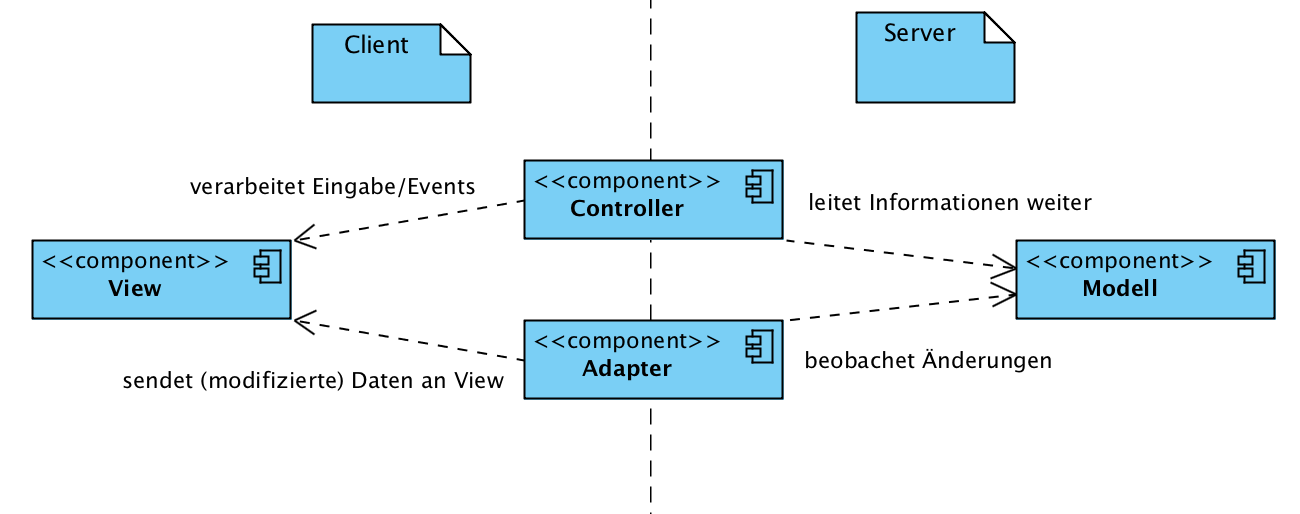
\includegraphics[width=1\textwidth]{MVC-Architektur}
	\caption[MVC]{Darstellung der MVC-Architektur mit Aufgaben}
	\label{fig:MVC}
\end{figure}
Hier wurde eine klassische Interpretierung des MVC-Musters gewählt, bei der der Controller lediglich Informationen aus Events der View verarbeitet und an das Modell weiterleitet. Für den zweiten Kommunikationsweg vom Modell zur View wurde eine separat zu implementierende Komponente gewählt: Der Adapter.
In der Mitte der Abbildung \ref{fig:MVC} ist eine Trennlinie zu erkennen. Sie soll die physische, sowie logische Grenze zwischen der Server- und der Client-Komponente repräsentieren. Auch zu erkennen ist, dass Controller und Adapter über diese Grenzen hinweg operieren müssen. Die View befindet sich auf dem Client und bekommt Benutzereingaben und soll möglichst aktuelle Daten aus dem Modell zur Anzeige bringen. Währenddessen befindet sich das Datenmodell des Spiels auf dem Server und implementiert die Regeln den Spiels, die für eine Integrität der Daten sorgen. Nun gibt es die Möglichkeit, dass der Controller komplett auf dem Client implementiert wird. Dies bringt den Vorteil, dass eine einzige Klasse an einer Position im Code hat, die für einen Kommunikationsweg zuständig ist. Der große Nachteil kommt jedoch auf der Server-Seite zum tragen: Hier muss das Modell stark an die Nachrichten des Controllers binden und Kommunikation im Datenmodell durchführen.  
Wenn dagegen der geteilte Ansatz eines Controller-Senders und -Empfängers gewählt wird, bleiben Nachrichten, also Kommunikation, auch in Klassen, die für Kommunikation zuständig sind und müssen nicht in anderen Klasse verarbeitet werden. Als Nachteil dieses Ansatzes ergibt sich der erhöhte Aufwand bei der Erstellung einer zusätzlichen Klasse. Die Vor- und Nachteile der Ansätze für den Entwurf des Controllers sind vollständig übertragbar auf den Adapter. Es wurde sich im Folgenden für den Ansatz der geteilten Controller und Adapter entschieden, sodass sich 4 Klassen zur Kommunikation zwischen Ansicht und Datenmodell ergeben: Jeweils ein Controller und ein Adapter auf Server- \bzw
Client-Seite. Die Aufgaben der Klassen sind bereits in Abbildung \ref{fig:MVC} an den Pfeilen abzulesen.\\
Aus den Anpassungen für die Kommunikation ergibt sich damit der Aufbau aus Abbildung \ref{fig:ArchitekturSplit}.
\begin{figure}[htp]
	\centering
	\captionsetup{justification=centering}
	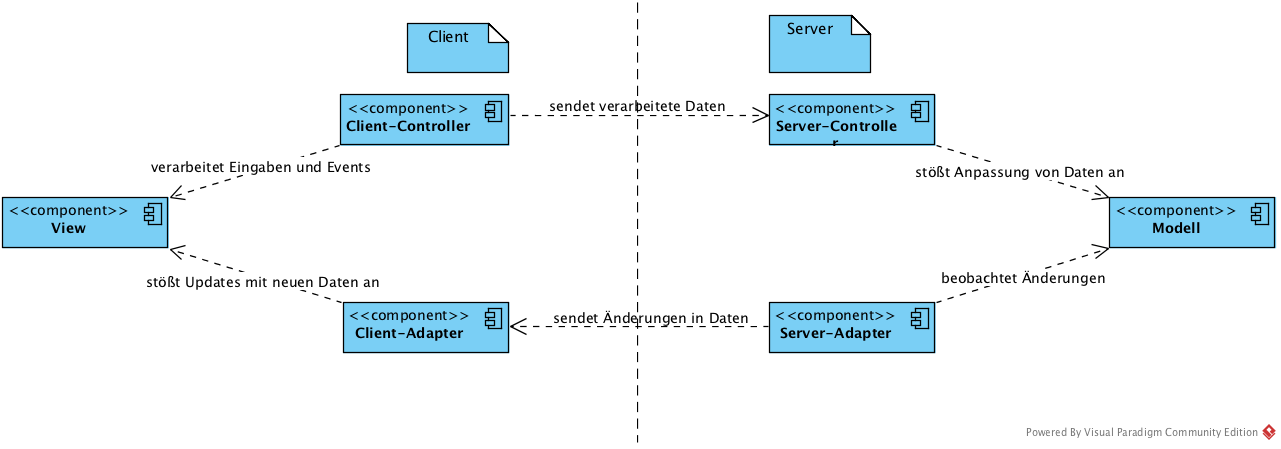
\includegraphics[width=1\textwidth]{BasisArchitekturSplit}
	\caption[ArchitekturSplit]{Aufgeteilte Kommunikationsklassen}
	\label{fig:ArchitekturSplit}
\end{figure}

\noindent Da zur Kommunikation von Daten zwangläufig auch zu übertragende Daten gehören muss das Datenmodell so gestaltet werden, dass immer auf die aktuellen Daten zugegriffen werden kann. Außerdem müssen die Daten in einem Format vorliegen, dass eine Übertragung erlaubt. Da gleichzeitig lesender Zugriff im Client und schreibender Zugriff im Server auf die komplette Datenhaltung möglich sein muss, bietet es sich an ein zentrales Modell aufzustellen. Das zentrale Modell wird dann in einem Initialzustand vom Server an den Client gesendet. Im Spielbetrieb müssen dann nur noch Aktualisierungen übertragen werden, was die Last der Kommunikationswege deutlich reduziert. Da das Datenmodell stark an das, eingangs dieses Kapitels, aufgestellte Begriffsmodell angelehnt sein muss, ist schnell ersichtlich welche Menge an Daten und auch welche Daten vorgehalten werden müssen.
Die Abbildung \ref{fig:InfoModel} zeigt die gewählten Daten-Schnittstellen für das Datenmodell. 
\begin{figure}[htp]
	\centering
	\captionsetup{justification=centering}
	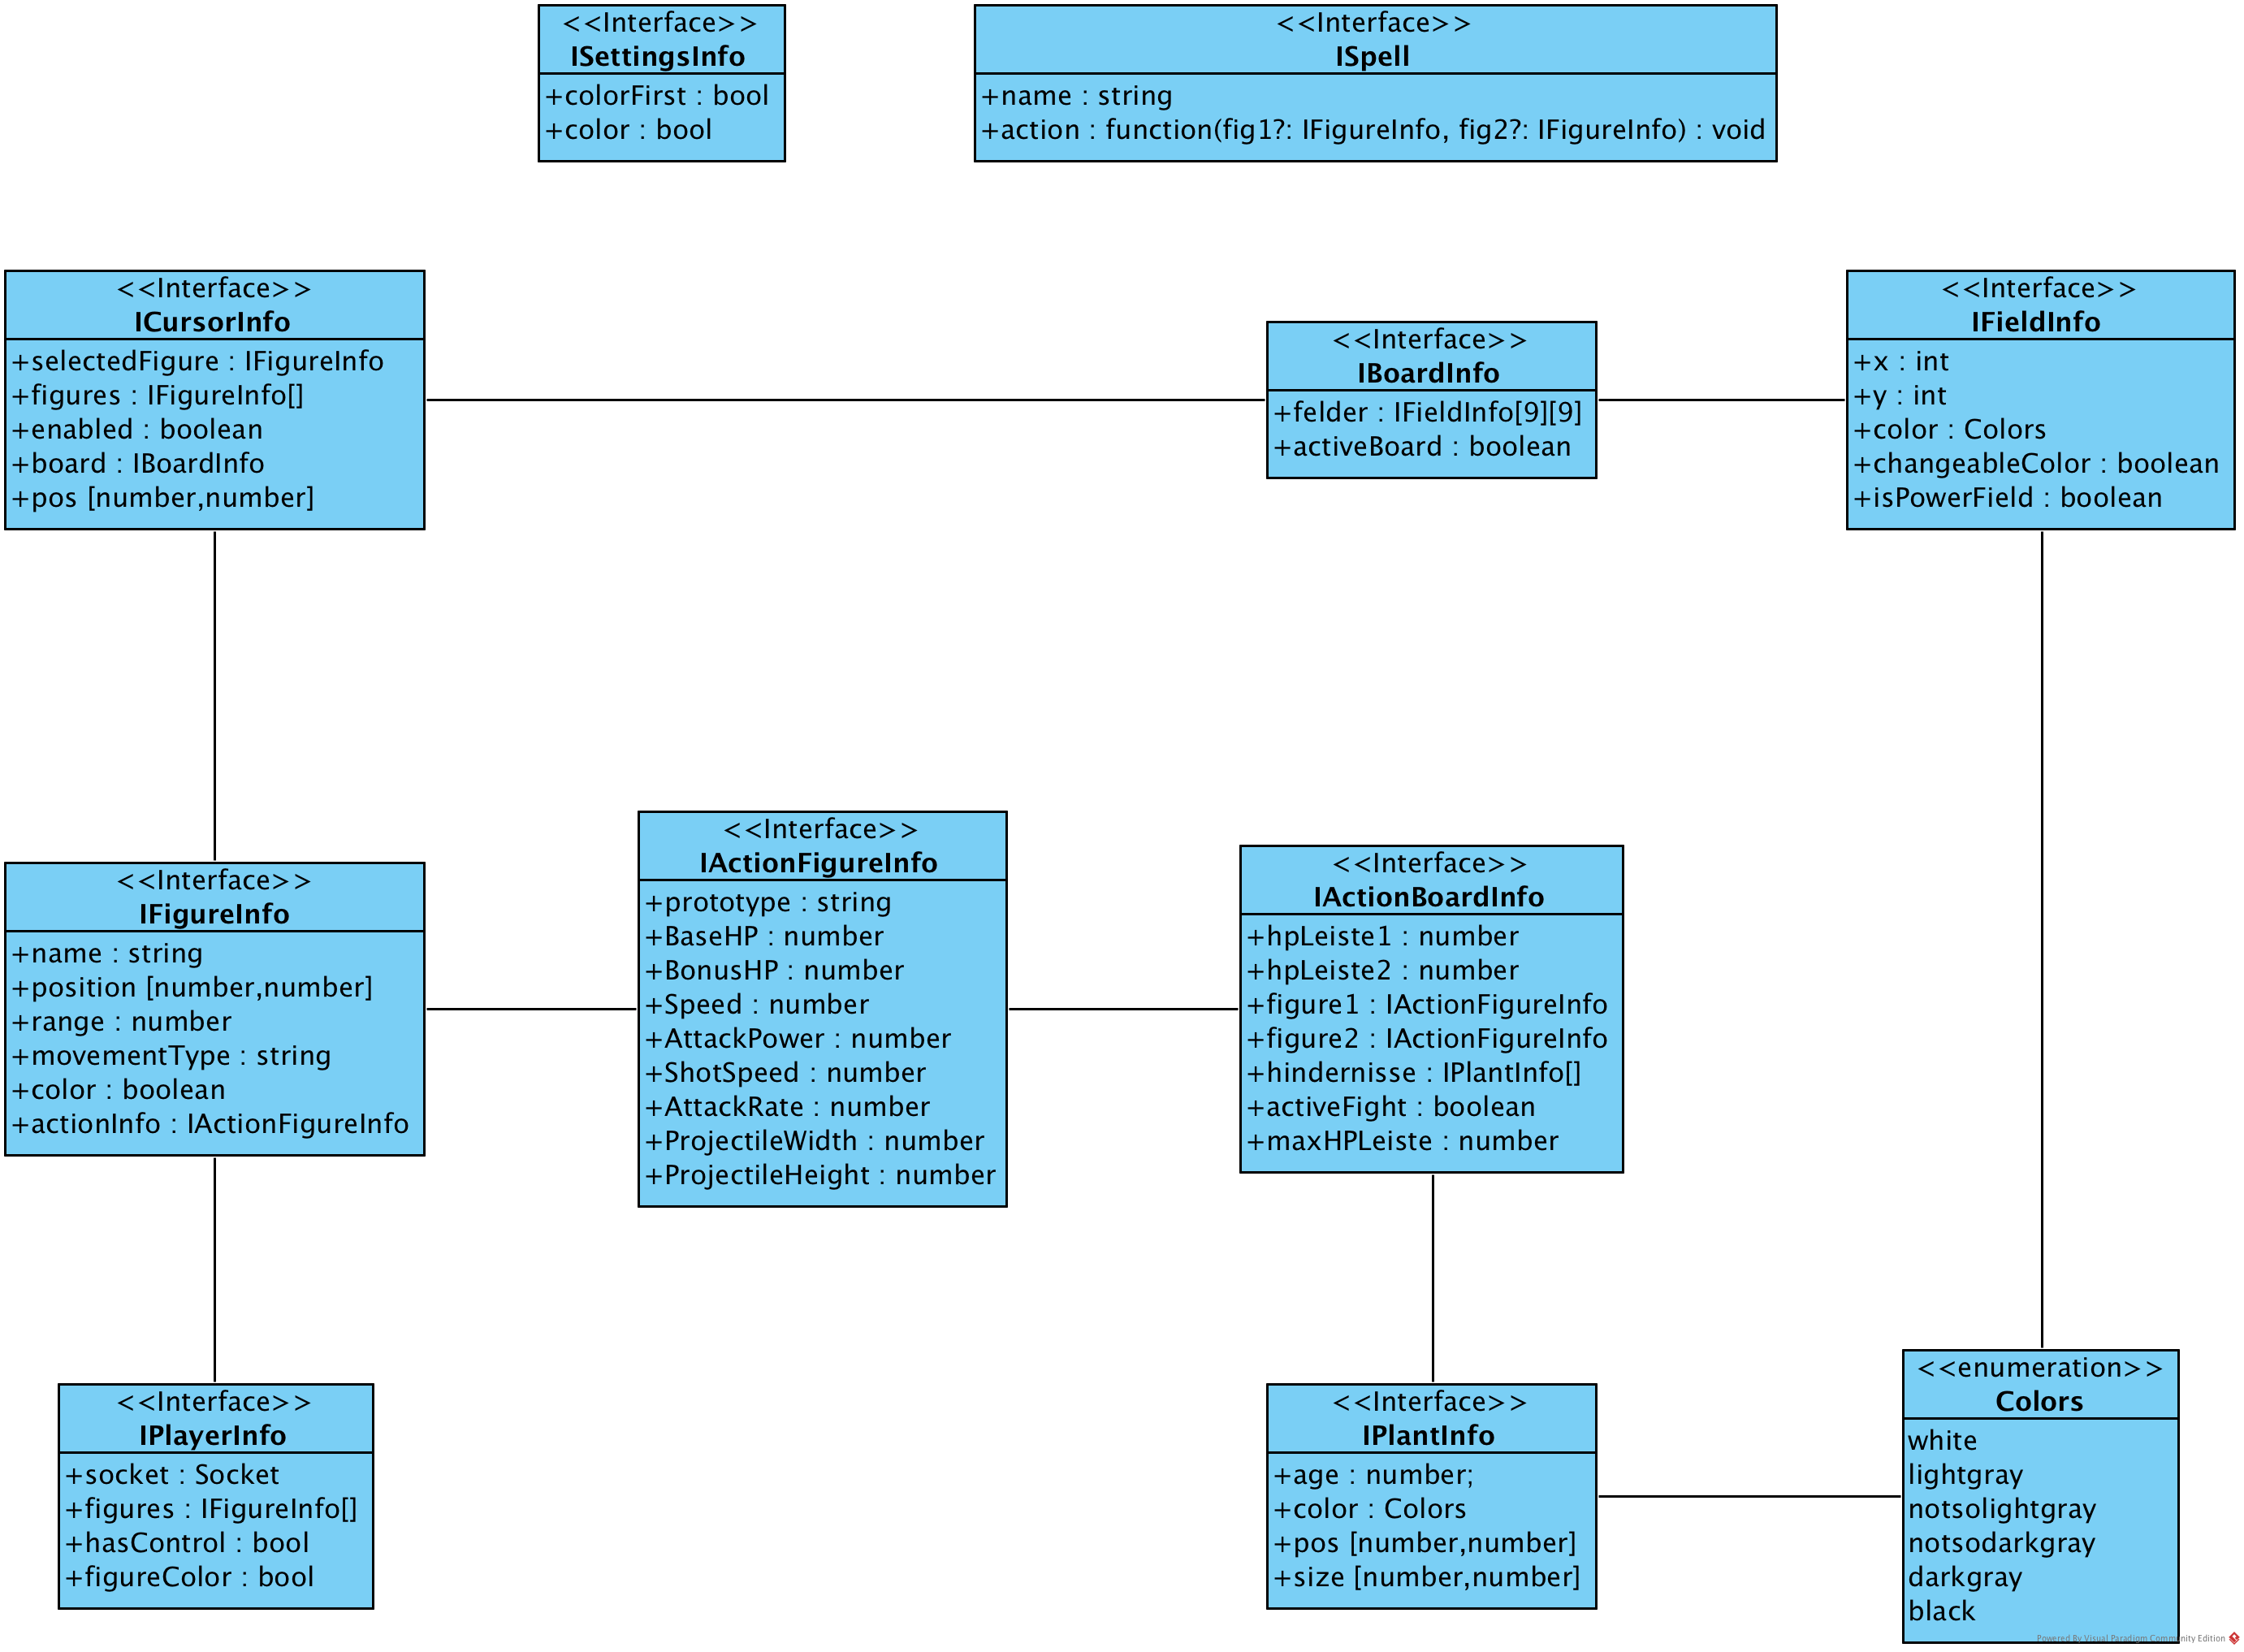
\includegraphics[width=0.9\textwidth]{InfoModel}
	\caption[InfoModel]{Daten-Schnittstellen für Datenmodell}
	\label{fig:InfoModel}
\end{figure}
\clearpage
\noindent Die Daten-Schnittstellen enthalten keine Methoden. Sie sind nur Container \bzw Verträge für Daten. Die Schnittstellen für die Einstellungen und die Zauber besitzen keine direkten Beziehungen zu den anderen Schnittstellen, sondern stellen ihre Beziehungen erst durch die Regeln des Spiels her. Die Ausarbeitung der Daten für die einzelnen Schnittstellen ergibt sich aus dem Begriffsmodell und der Beschreibung des Spiels. Die meisten Schnittstellen werden zur gebündelten Übertragung in der Schnittstelle IGameModel vereint:


\begin{figure}[htp]
	\centering
	\captionsetup{justification=centering}
	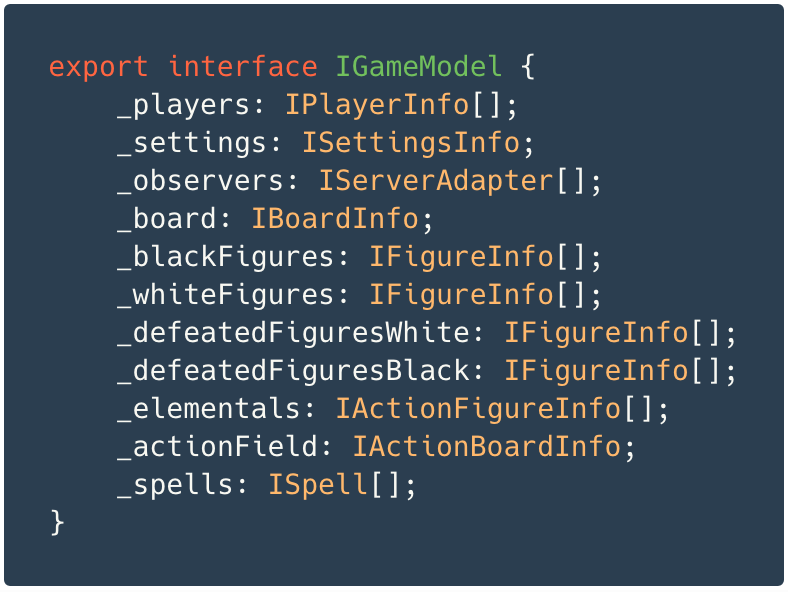
\includegraphics[width=0.6\textwidth]{IGameModel}
	\caption[IGameModel]{Daten-Schnittstelle IGameModel}
	\label{fig:IGameModel}
\end{figure}
\noindent Zu jeder Daten-Schnittstelle fehlen jetzt noch die passenden Klassen für Anzeige und Logik um die wesentlichen Teile der Grobarchitektur fertigzustellen. Zu jeder Info-Schnittstelle gibt es also zwei weitere Klassen \zB zur IBoardInfo-Schnittstelle die Klassen Board für Spiellogik im Server und BoardView zur Anzeige im Client. Die Komponenten View und Modell werden im Folgenden nacheinander vorgestellt.
\clearpage
\subsubsection{View}
\begin{figure}[htp]
	\centering
	\captionsetup{justification=centering}
	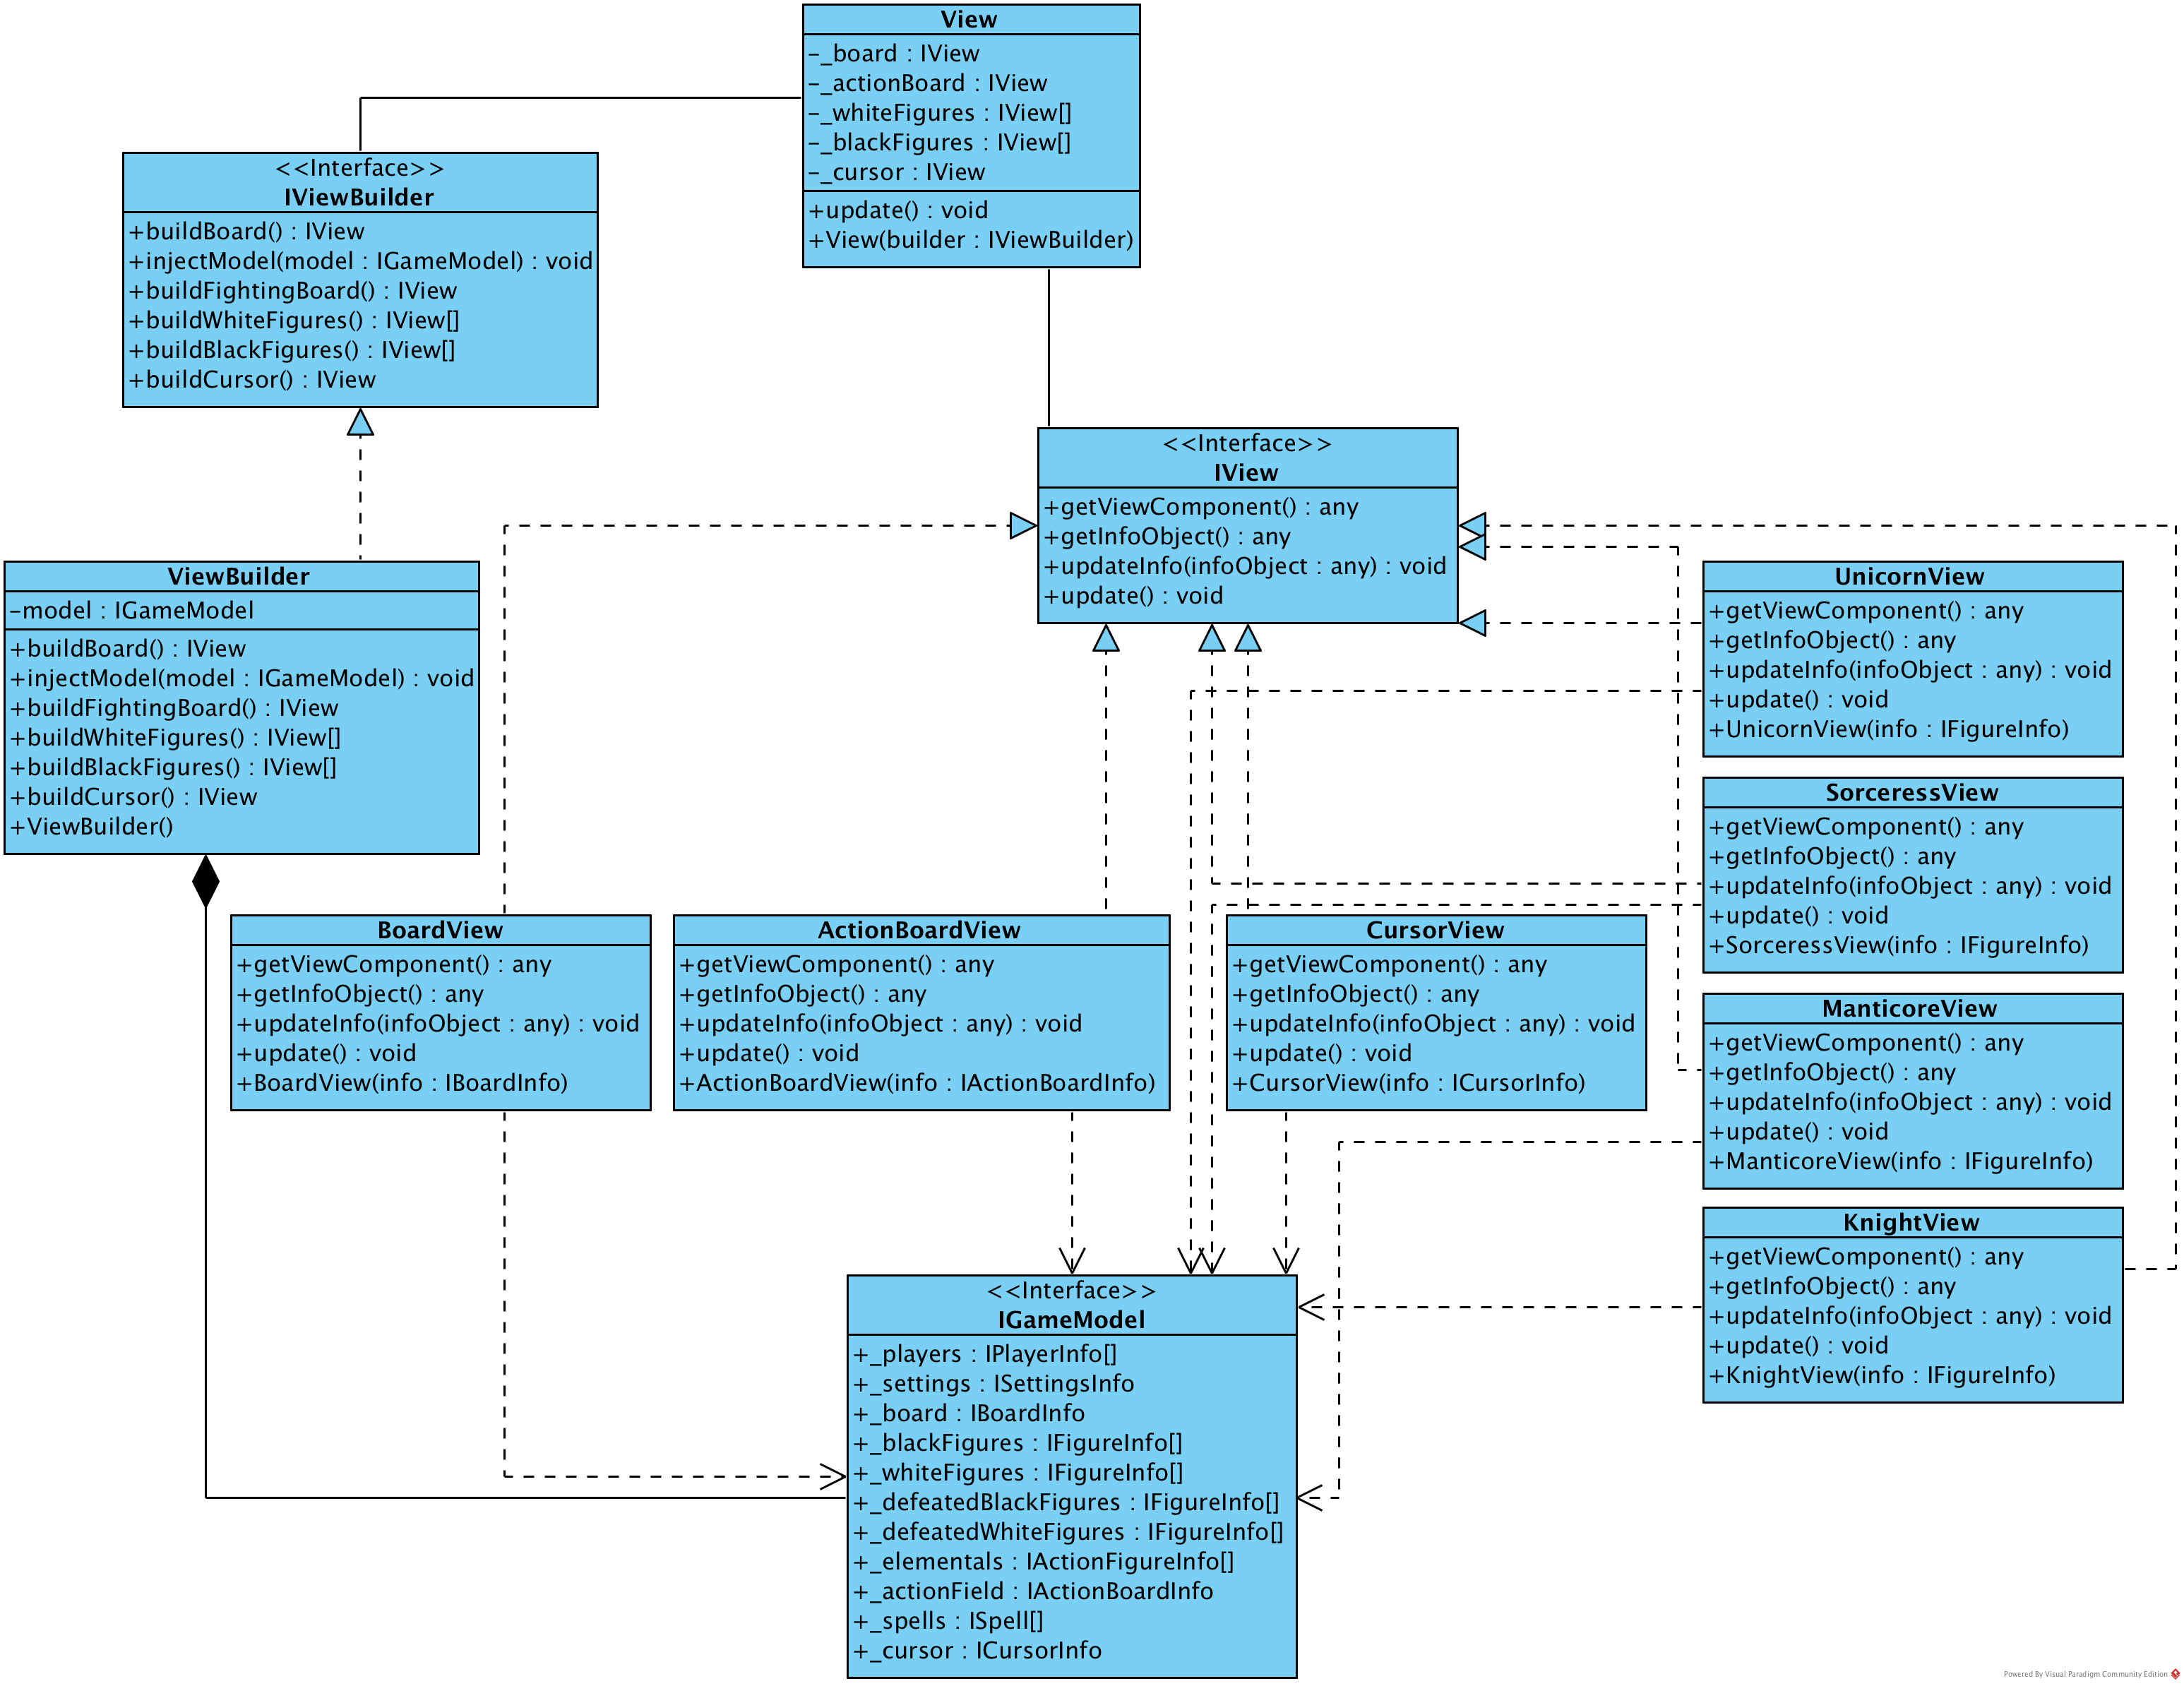
\includegraphics[width=1\textwidth]{View_Class_Diagram}
	\caption[View]{leicht vereinfachtes Klassendiagramm der View}
	\label{fig:ClassesView}
\end{figure}

\noindent Die Abbildung \ref{fig:ClassesView} zeigt eine leicht vereinfachte Darstellung der View-Komponente. Die Vereinfachungen bestehen in der reduzierten Darstellung der Anzeige-Klassen für die einzelnen Figurentypen. Exemplarisch sind hier nur die Typen "Knight", "Manticore", "Sorceress" und "Unicorn" dargestellt, da sich die Klassen nur in der Implementierung ihres Konstruktors unterscheiden, der das eigentliche 3D-Objekt anhand eines Informationsobjektes aus dem Datenmodell erzeugt.\\
Für den "ViewBuilder" wurde der Ansatz einer Injektionsmethode zur Anbindung an das Datenmodell gewählt. Damit kann die Objekt-Erzeugung vom Zeitpunkt der Injektion der Abhängigkeit entkoppelt werden. Das ist hier sinnvoll, da das Datenmodell zu einem Zeitpunkt zum Client gesendet wird, den dieser nicht beeinflussen kann. Der "ViewBuilder" hat die Aufgabe die einzelnen Erzeugungen von Anzeigeobjekten von der View zu entkoppeln, was den einfacheren Tausch eines Frameworks für die 3D-Objekte erlaubt und die bessere Bündelung von Abhängigkeiten möglich macht. Außerdem entkoppelt er die View von der Kenntnis über ein Datenmodell, sodass diese lediglich Anzeigeobjekte besitzt und auch nur für deren Aktualisierungen und tatsächliche Anzeige zuständig ist.\\
Desweiteren besitzen alle Anzeigeklassen eine Referenz auf ihr Informationsobjekt aus dem Datenmodell, sodass der Adapter Änderungen nur in das Modell auf dem Client laden muss und die View alle ihre Anzeigeobjekte in einer Schleife regelmäßig zu Aktualisierungen auffordert. Die einzelnen Anzeigeklassen interpretieren dabei die Informationen aus ihren Datenobjekten und wandeln diese in eine passende Darstellung basierend auf dem gewählten 3D-Framework.\\

\subsubsection{Modell}
\begin{figure}[htp]
	\centering
	\captionsetup{justification=centering}
	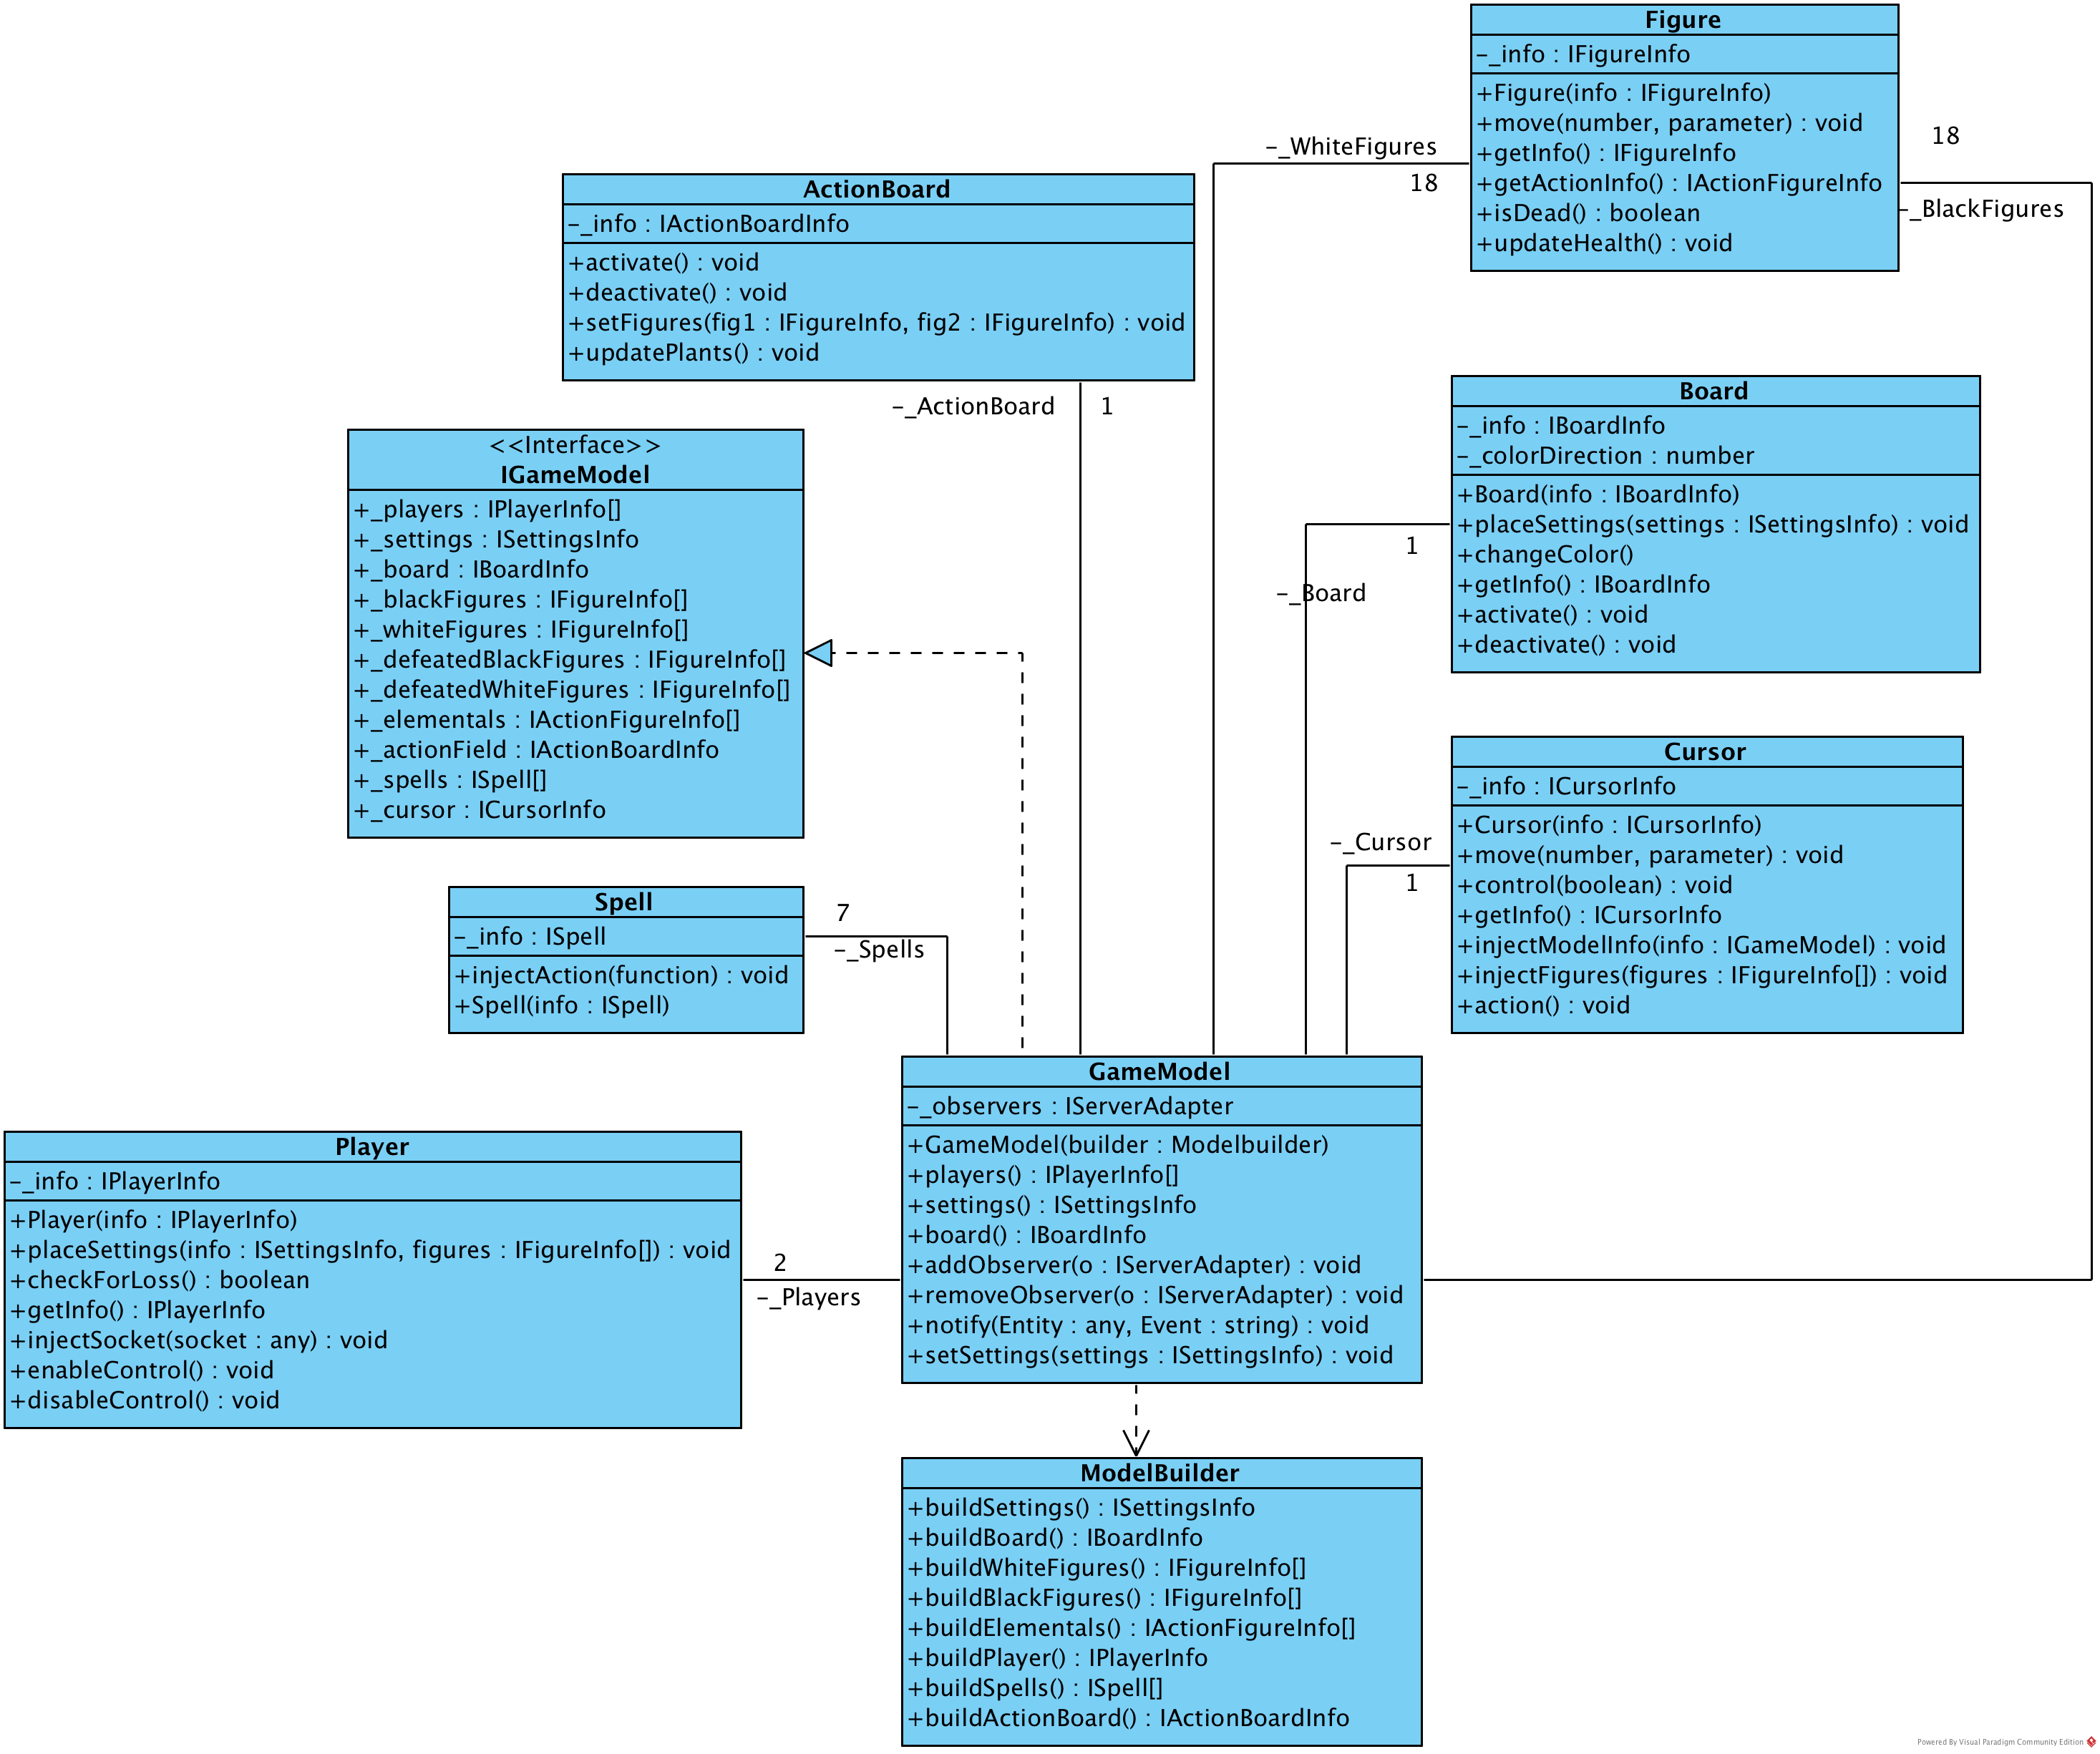
\includegraphics[width=1\textwidth]{Modell_Class_Diagram}
	\caption[Modell]{Klassendiagramm des Modells}
	\label{fig:ClassesModell}
\end{figure}

\noindent Das Modell wurde sehr ähnlich zur View strukturiert. Die Klasse "ModelBuilder" ist für die korrekte Erzeugung eines Initialzustandes des Datenmodells zuständig. Während die Klasse "GameModel" die Erzeugung der Logik-Objekte selbst übernimmt, da diese keine aufwändigen Initialisierungsroutinen besitzen. Jedes Logik-Objekt kann auf sein Informationsobjekt zugreifen und besitzt Methoden zum Schreiben der Daten. Die Methoden sind dabei zuständig für das Überprüfen von Spielregeln, wie die Reichweite von Figuren, oder das Ändern der Farbe der Felder auf dem Spielbrett.\\
An dieser Stelle sei noch die Implementierung des Beobachter-Musters zu erwähnen. Die Klasse "GameModel" muss den Adapter nach der Änderung von Daten informieren können, sodass der Adapter die geänderten Daten an den Client senden kann. Dafür trägt sich der Adapter in die Liste der Beobachter im "GameModel" ein und wird anschließend mittels der "notify"-Methode vom "GameModel" darüber benachrichtigt welche Daten sich geändert haben und kann die Änderungen einfach weiterleiten.

Da nun alle wesentlichen Komponenten des System beschrieben wurden, bleibt nun lediglich die Ansicht der technologischen Abhängigkeiten zu zeigen.

\subsubsection{Abhängigkeiten}
\begin{figure}[htp]
	\centering
	\captionsetup{justification=centering}
	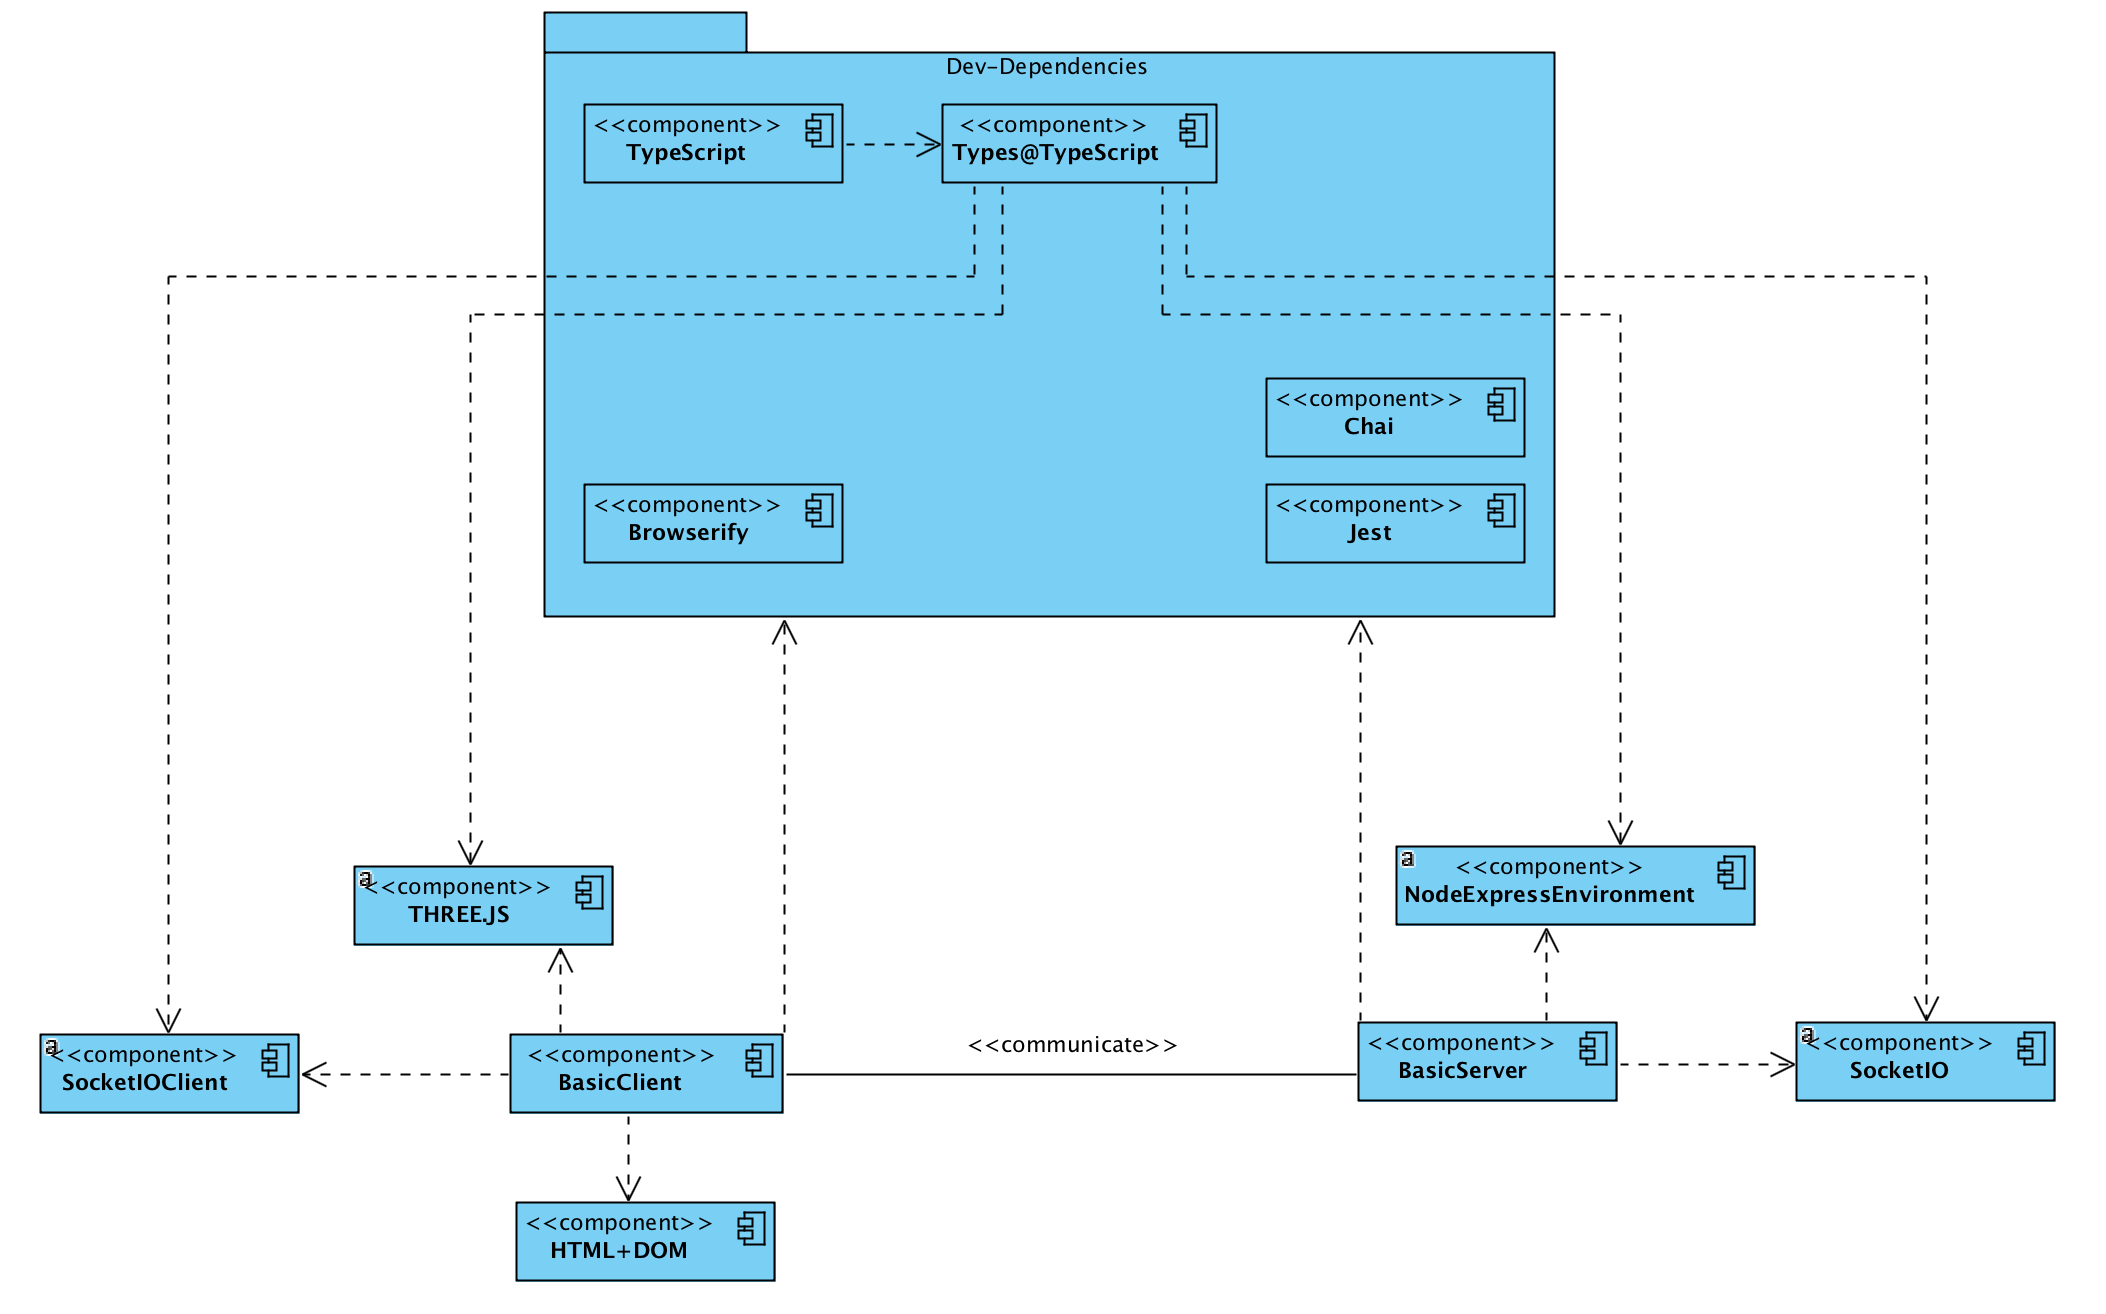
\includegraphics[width=1\textwidth]{Dependencies}
	\caption[Abhängigkeiten]{Komponentendiagramm der Abhängigkeiten}
	\label{fig:ComponentDependencies}
\end{figure}
\noindent Die Grafik \ref{fig:ComponentDependencies} zeigt eine Übersicht über die Abhängigkeiten des Servers und des Clients zu den gewählten Frameworks und Software-Bibliotheken. Da deren Verwendung schon in Kapitel \ref{subsec:Technologien} \bzw \ref{subsec:Hilfsmittel} erläutert wurde dient diese Übersicht nur noch einmal zur Visualisierung und als Einstieg für die Implementierung der Architektur im folgenden Abschnitt.
\subsection{Schritte der Implementierung}
\label{subsec:Implementierung}\index{Implementierung}
Bei der Implementierung wurde sich zunächst mit den einzelnen Technologien aus der Grafik \ref{fig:ComponentDependencies} vertraut gemacht. Dafür wurden verschiedene Beispiele herangezogen und die Dokumentation, sowie \ggf vorhandene Getting-Started-Guides durchgearbeitet.\footnote{So zum Beispiel für Socket.IO: \url{https://socket.io/get-started/chat/}}
Anschließend wurde die Entwicklungsumgebung aufgesetzt auf Basis eines Starter-Projektes für Node.js-Projekte mit Typescript und Express.\cite{typescript_node_starter} Dabei wurde das Starter-Projekt so angepasst, dass die Applikation auf das Bereitstellen von statischen Webseiten spezialisiert ist. Einige Skripte zum Erstellen, Debuggen, Bündeln und Minimieren der Applikation wurden angepasst \bzw hinzugefügt. Der Aufbau des Projektes wird im Folgenden näher erläutert.
Generell ist ein solches Projekt mit Node.js immer auf einer Datei mit dem Namen "package.json" aufgebaut. Diese Datei enthält neben wichtigen Meta-Informationen, wie dem Namen des Projektes und seiner Version, auch Informationen, wie bestimme Befehle wie ein Start, das Debuggen \etc ausgeführt werden sollen. Auch sind in dieser Datei die Abhängigkeiten und die Entwicklungs-Abhängigkeiten enthalten. Dabei wird ein Paket immer mit seiner benutzen Version angegeben und möglichst große Portabilität zu erreichen und einen Projekt-Stand exakt reproduzieren zu können.

\section{Resultate}
\label{sec:Resultate}\index{Resultate}

\emph{Hier soll dann ein Screenshot des Ergebnisses rein und erläutert werden, dass als nächste der Endstand mit seiner Architektur gezeigt wird und anschließend die Erfüllung aller Anforderungen sichergestellt wird. Als letztes (falls genug Zeit!) werden die (hoffentlich) programmierten Unit-Tests erwähnt, und deren Ergebnisse dargestellt.}

\subsection{Überprüfung der Software mit Unit-Tests}
\label{subsec:unittests}\index{Unittests}

\emph{Hier wird dann die breite der Unit-Tests gezeigt, deren Anzahl und die Beschränkungen, also Code-Abdeckung. Anschließend ein Ergebnis-Log von einem Lauf auf dem finalen Stand.}

\subsection{Erfüllung der Anforderungen}
\label{subsec:erfullung_anforderungen}\index{Erfüllung}

\emph{Hier werden die Anforderungen aus dem Analyse-Teil aufgegriffen und mit der fertigen Anwendung und ihrer Architektur abgeglichen, also so was wie "die einzelnen Figuren und ihre Unterschiede, sind hier und hier da und da durch umgesetzt worden."}

\section{Fazit}
\label{sec:Fazit}\index{Fazit}
% !TeX root = ../Bachelorarbeit.tex

\chapter{Fazit und Ausblick}
\label{cha:fazit}

\emph{Die Ergebnisse wurden bisher nur dargestellt und erklärt und nicht bewertet und analysiert, dass soll hier geschehen unter "erreichte Ziele". Das Fazit soll Punkte zu Anwendbarkeit der Technologien, Entwicklung/Nachbau eines Spieleklassikers und Problempunkte, aber auch positives zu Support und Inbetriebnahme enthalten. Der Ausblick soll kommende Technologien und weitere Entwicklungspunkte für das Spiel beleuchten.}

\section{Fazit}
\label{sec:Schlussfolgerung}\index{Fazit}

\subsection{erreichte Ziele}
\label{subsec:erreichte_ziele}

\section{Ausblick}
\label{sec:Ausblick}\index{Ausblick}

Die Entwicklung dieses Ablegers von Archon ist keinesfalls abgeschlossen. Es gibt viele offene Features und Themen für weitere Abschlussarbeiten.

\subsubsection{Generelle Weiterentwicklung}

Das Spiel an sich ist noch nicht komplett reproduziert worden.

\subsubsection{KI-Modus / Demo-Modus}

Diese Realisierung hat bisher nur menschliche Spieler realisiert, jedoch erlaubt die Architektur genauso den Ersatz der View-Komponente durch einen Computer-Spieler. Eine spannende Arbeit kann daher die Entwicklung einer künstlichen Intelligenz (KI) für den Demo-Modus \bzw den Modus Spieler-vs-Computer sein.

\subsubsection{Score-Boards}

Es können eine Datenbank und ein Authentifizierungsservice angebunden werden und damit Spieler registriert werden. Das würde die Implementierung einer Rangliste (Score-Board) oder eines Systems von Spielerfolgen (Achievements) ermöglichen.

\subsubsection{Verschiedenes}
\cleardoublepage

% Anhang -----------------------------------------------------------------------
%   Die Inhalte des Anhangs werden analog zu den Kapiteln inkludiert.
%   Dies geschieht in der Datei "Anhang.tex".
% ------------------------------------------------------------------------------
\addtocontents{toc}{\protect\newpage} %Seitenumbruch in Inhaltsverzeichnis erzwingen

\begin{appendix}
    \clearpage
    %\pagenumbering{Roman}
    %\pagenumbering{arabic}
    \renewcommand{\thepage}{\thechapter-\arabic{page}}
    \setcounter{page}{1}
    %\setcounter{page}{\pageref{inhalt_ende}}
    % Rand der Aufzählungen in Tabellen anpassen
    %\setdefaultleftmargin{1em}{}{}{}{}{}
    % !TeX root = ../Bachelorarbeit.tex
\chapter{Anhang - Informationen zu Tools}
\label{cha:Anhang_Info}

\section{Erweiterungen von Visual Studio Code}
\label{sec:extensions}
Die installierten Erweiterungen des Editors Visual Studio Code werden folgend alphabetisch aufgelistet: 
\begin{multicols}{2}
	\begin{itemize}
		\item alefragnani.project-manager
		\item austin.code-gnu-global
		\item christian-kohler.path-intellisense
		\item dbaeumer.vscode-eslint
		\item donjayamanne.githistory
		\item eamodio.gitlens
		\item eg2.tslint
		\item formulahendry.code-runner
		\item James-Yu.latex-workshop
		\item mitaki28.vscode-clang	
	\end{itemize}
	\columnbreak
	\begin{itemize}
		\item ms-vscode.azure-account
		\item ms-vscode.cpptools
		\item ms-vscode.csharp
		\item msjsdiag.debugger-for-chrome
		\item redhat.java
		\item robertohuertasm.vscode-icons
		\item rokoroku.vscode-theme-darcula
		\item streetsidesoftware.code-spell-checker
		\item streetsidesoftware.code-spell-checker-german
		\item WallabyJs.wallaby-vscode
		\item zhuangtongfa.Material-theme
	\end{itemize}
\end{multicols}

\section{weitere Diagramme}
\label{sec:additionalDiagrams}

\begin{figure}[htp]
	\centering
	\captionsetup{justification=centering}
	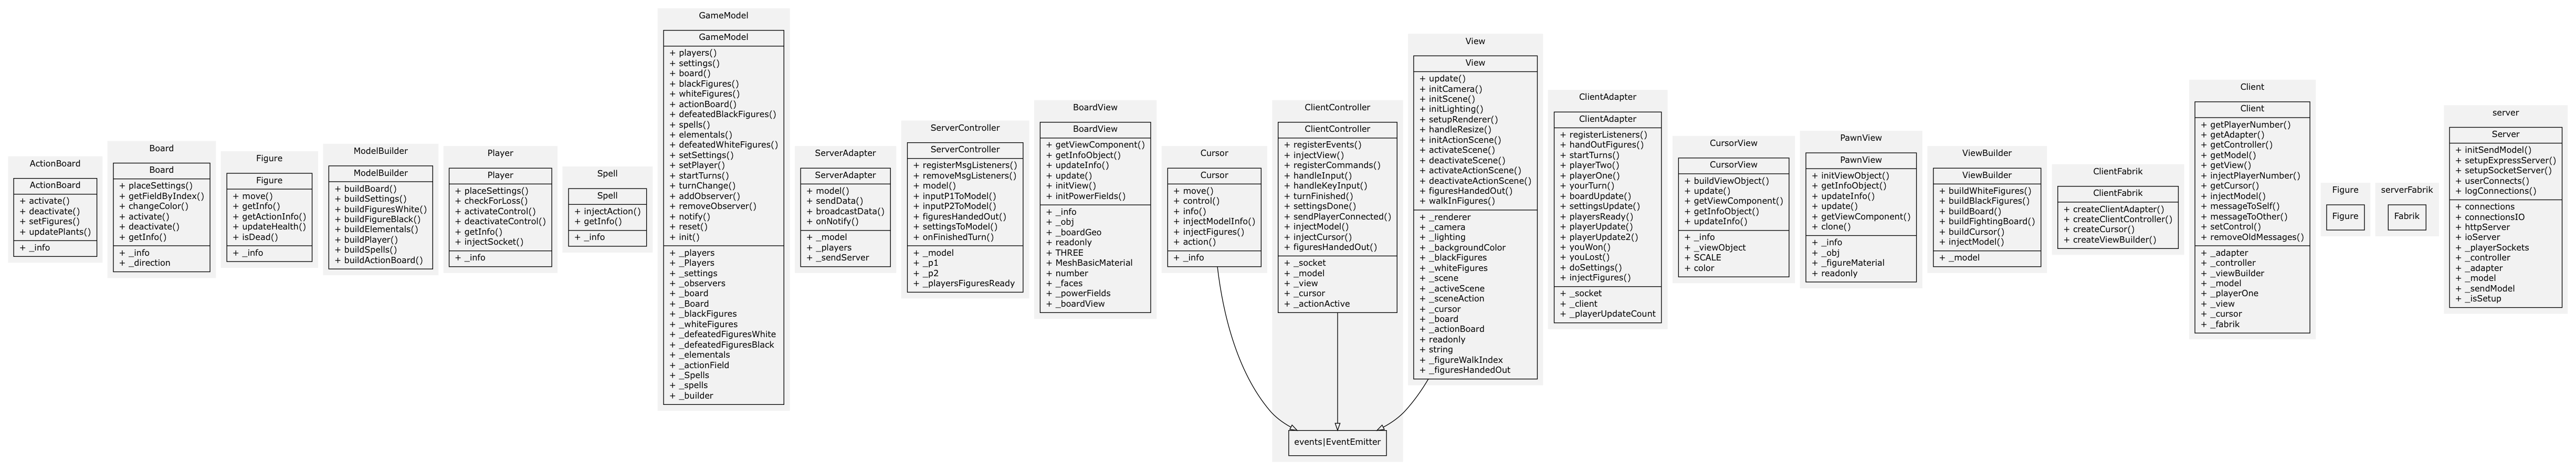
\includegraphics[width=1\textwidth]{Overview}
	\caption[Überblick Klassen]{Eine Übersicht über die implementierten Klassen}
	\label{fig:overviewClasses}
\end{figure}

\begin{figure}[htp]
	\centering
	\captionsetup{justification=centering}
	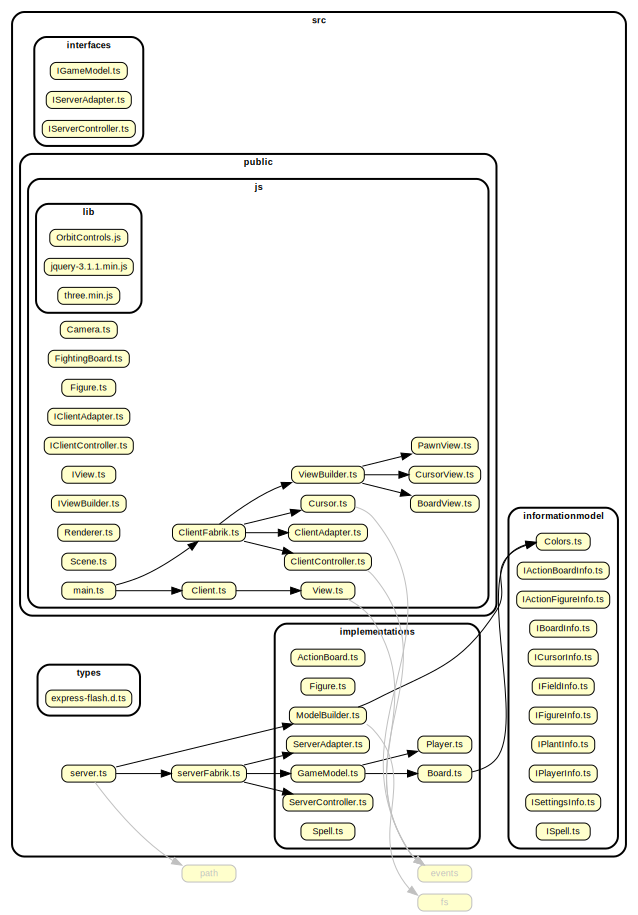
\includegraphics[width=1\textwidth]{dependencygraph}
	\caption[Überblick Abhängigkeiten]{Eine Übersicht über die Abhängigkeiten}
	\label{fig:overviewDep}
\end{figure}

\section{Ordnerstruktur der CD}
\label{sec:treeCD}

\begin{figure}[htp]
	\centering
	\captionsetup{justification=centering}
	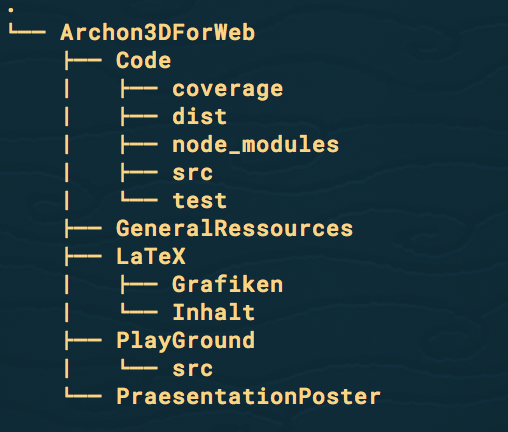
\includegraphics[width=0.45\textwidth]{TreeCD}
	\caption[Ordnerstruktur CD]{Ordnerstruktur der CD}
	\label{fig:TreeCD}
\end{figure}
    \cleardoublepage
\end{appendix}


% Verzeichnis ---------------------------------------------------------
\setlength{\parindent}{0pt}
\pagenumbering{Roman}
\setcounter{page}{\thetocPage} % echten Seitenzähler ändern

%\addcontentsline{toc}{chapter}[\arabic{chapter}.Verzeichnisse]{Verzeichnisse}
\cleardoublepage\phantomsection
\addcontentsline{toc}{chapter}{Verzeichnisse}
%\addcontentsline{toc}{chapter}[\arabic{chapter}.Verzeichnisse]{Verzeichnisse}
%\addcontentsline{toc}{chapter}{\texorpdfstring{\arabic{chapter}.Verzeichnisse}{Verzeichnisse}} % wegen PDF Verweisen

% Literaturverzeichnis ---------------------------------------------------------
% Das Literaturverzeichnis wird aus der BibTeX-Datenbank "Bibliographie.bib" erstellt.
\cleardoublepage\phantomsection
\markboth{\refname}{\refname} % f�r korrekte �berschrift in der Kopfzeile
\addcontentsline{toc}{section}{\refname}
%\bibliographystyle{dinat}
%\bibliographystyle{alphadin}
\bibliographystyle{natdin} % DIN-Stil des Literaturverzeichnisses
\bibliography{Bibliographie} % Aufruf: bibtex Masterarbeit

% Abbildungsverzeichnis --------------------------------------------------------
\cleardoublepage\phantomsection
\markboth{\listfigurename}{\listfigurename} % f�r korrekte �berschrift in der Kopfzeile
\addcontentsline{toc}{section}{\listfigurename}
\listoffigures

% Tabellenverzeichnis ---------------------------------------------------------
\cleardoublepage\phantomsection
\markboth{\listtablename}{\listtablename} % f�r korrekte �berschrift in der Kopfzeile
\addcontentsline{toc}{section}{\listtablename}
\listoftables

% Code Listen Verzeichnis ------------------------------------------------------
\cleardoublepage\phantomsection
\markboth{\lstlistlistingname}{\lstlistlistingname} % f�r korrekte �berschrift in der Kopfzeile
\addcontentsline{toc}{section}{\lstlistlistingname}
\lstlistoflistings % Listings-Verzeichnis

% Verzeichnisstruktur der DVD -------------------------------------------------
\newpage
\cleardoublepage
\include{Inhalt/VerzeichnissStruktur}

% Abkürzungsverzeichnis -----------------------------------------------------
\cleardoublepage\markboth{\nomname}{\nomname} % f�r korrekte �berschrift in der Kopfzeile
\phantomsection
\addcontentsline{toc}{section}{\nomname}
\abk{o.V.}{ohne Verfasser (bei Literaturverweisen)}
\abk{Abb.}{Abbildung}
\abk{API}{Programmschnittstelle nach aussen (engl. f{\"u}r Application Programming Interface)}
\abk{SDK}{\sa IDE (engl f{\"u}r Software Development Kit)}
\abk{IDE}{integrierte Entwicklungsumgebung (engl. f{\"u}r Integrated Development Environment)}

\abk{W3C}{Organisation zur Standardisierung von Webtechnologien (engl. f{\"u}r World Wide Web Consortium)}
\abk{WWW}{Internet (engl. f{\"u}r World Wide Web)}
\abk{DOM}{Dokumentstruktur der Webseite (engl. f{\"u}r Document Object Model)}
\abk{HTML}{Hypertext Auszeichnungssprache, HTML-Dateien sind die Grundlage des World Wide Web und werden von einem Webbrowser dargestellt (engl. f{\"u}r Hypertext Markup Language)}
\abk{HTTP}{Hypertext-\"Ubertragungsprotokoll, Protokoll zur \"Ubertragung von Daten \"uber ein Netzwerk  (engl. f{\"u}r Hypertext Transfer Protocol)}
\abk{HTTPS}{sicheres Hypertext-\"Ubertragungsprotokoll \sa HTTP (engl. f\"ur Hypertext Transfer Protocol Secure)}
\abk{Webseite}{\sa HTML-Datei}
\abk{CSS}{gestufte Gestaltungsb\"ogen, legt die Darstellung des HTML Quellcodes im Browser fest (engl. f{\"u}r Cascading Style Sheets)}
\abk{JavaScript}{Skriptsprache, urspr\"unglich f\"ur dynamisches HTML in Webbrowsern entwickelt}
\abk{JSON}{kompaktes Datenformat zum Datenaustausch mit \zB Webservern (engl. f{\"u}r JavaScript Object Notation)}
\abk{Webbrowser}{auch kurz Browser (engl. to browse) steht f{\"u}r durchst{\"o}bern, abgrassen, durchsuchen - Software zum Darstellen von Daten, haupts{\"a}chlich Webseiten und deren Inhalt, k\"onnen zu diesem Zweck mit Webservern kommunizieren}
\abk{Webserver}{Ein Webserver speichert Webseiten und stellt diese zur Verf\"ugung. Der Webserver ist eine Software, die Dokumente mit Hilfe standardisierter \"Ubertragungsprotokolle (HTTP, HTTPS) an einen Webbrowser \"ubertr\"agt.}
\abk{GUI}{Grafisches Benutzer Interface (engl. f{\"u}r Graphical User Interface)}
\abk{Interface}{Schnittstelle}
\abk{JPEG}{komprimierte Grafikdatei, auch JPG (engl. f\"ur Joint Photographic Expert Group)}
\abk{GIF}{Grafikaustausch Format, Animationsf\"ahig (engl. f\"ur Graphics Interchange Format)}
\abk{PNG}{Grafikaustausch Format (engl. f\"ur Portable Network Graphics)}
\abk{SVG}{skalierbare Vektorgrafik (engl. f\"ur Scalable Vector Graphics)}


\printnomenclature

% Stichwortverzeichnis ---------------------------------------------------------
\cleardoublepage\markboth{\indexname}{\indexname} % f�r korrekte �berschrift in der Kopfzeile
\phantomsection
\addcontentsline{toc}{section}{\indexname}
\printindex

\end{document}
